\documentclass[11pt]{article}

    \usepackage[breakable]{tcolorbox}
    \usepackage{parskip} % Stop auto-indenting (to mimic markdown behaviour)
    
    \usepackage{iftex}
    \ifPDFTeX
    	\usepackage[T1]{fontenc}
    	\usepackage{mathpazo}
    \else
    	\usepackage{fontspec}
    \fi

    % Basic figure setup, for now with no caption control since it's done
    % automatically by Pandoc (which extracts ![](path) syntax from Markdown).
    \usepackage{graphicx}
    % Maintain compatibility with old templates. Remove in nbconvert 6.0
    \let\Oldincludegraphics\includegraphics
    % Ensure that by default, figures have no caption (until we provide a
    % proper Figure object with a Caption API and a way to capture that
    % in the conversion process - todo).
    \usepackage{caption}
    \DeclareCaptionFormat{nocaption}{}
    \captionsetup{format=nocaption,aboveskip=0pt,belowskip=0pt}

    \usepackage[Export]{adjustbox} % Used to constrain images to a maximum size
    \adjustboxset{max size={0.9\linewidth}{0.9\paperheight}}
    \usepackage{float}
    \floatplacement{figure}{H} % forces figures to be placed at the correct location
    \usepackage{xcolor} % Allow colors to be defined
    \usepackage{enumerate} % Needed for markdown enumerations to work
    \usepackage{geometry} % Used to adjust the document margins
    \usepackage{amsmath} % Equations
    \usepackage{amssymb} % Equations
    \usepackage{textcomp} % defines textquotesingle
    % Hack from http://tex.stackexchange.com/a/47451/13684:
    \AtBeginDocument{%
        \def\PYZsq{\textquotesingle}% Upright quotes in Pygmentized code
    }
    \usepackage{upquote} % Upright quotes for verbatim code
    \usepackage{eurosym} % defines \euro
    \usepackage[mathletters]{ucs} % Extended unicode (utf-8) support
    \usepackage{fancyvrb} % verbatim replacement that allows latex
    \usepackage{grffile} % extends the file name processing of package graphics 
                         % to support a larger range
    \makeatletter % fix for grffile with XeLaTeX
    \def\Gread@@xetex#1{%
      \IfFileExists{"\Gin@base".bb}%
      {\Gread@eps{\Gin@base.bb}}%
      {\Gread@@xetex@aux#1}%
    }
    \makeatother

    % The hyperref package gives us a pdf with properly built
    % internal navigation ('pdf bookmarks' for the table of contents,
    % internal cross-reference links, web links for URLs, etc.)
    \usepackage{hyperref}
    % The default LaTeX title has an obnoxious amount of whitespace. By default,
    % titling removes some of it. It also provides customization options.
    \usepackage{titling}
    \usepackage{longtable} % longtable support required by pandoc >1.10
    \usepackage{booktabs}  % table support for pandoc > 1.12.2
    \usepackage[inline]{enumitem} % IRkernel/repr support (it uses the enumerate* environment)
    \usepackage[normalem]{ulem} % ulem is needed to support strikethroughs (\sout)
                                % normalem makes italics be italics, not underlines
    \usepackage{mathrsfs}
    

    
    % Colors for the hyperref package
    \definecolor{urlcolor}{rgb}{0,.145,.698}
    \definecolor{linkcolor}{rgb}{.71,0.21,0.01}
    \definecolor{citecolor}{rgb}{.12,.54,.11}

    % ANSI colors
    \definecolor{ansi-black}{HTML}{3E424D}
    \definecolor{ansi-black-intense}{HTML}{282C36}
    \definecolor{ansi-red}{HTML}{E75C58}
    \definecolor{ansi-red-intense}{HTML}{B22B31}
    \definecolor{ansi-green}{HTML}{00A250}
    \definecolor{ansi-green-intense}{HTML}{007427}
    \definecolor{ansi-yellow}{HTML}{DDB62B}
    \definecolor{ansi-yellow-intense}{HTML}{B27D12}
    \definecolor{ansi-blue}{HTML}{208FFB}
    \definecolor{ansi-blue-intense}{HTML}{0065CA}
    \definecolor{ansi-magenta}{HTML}{D160C4}
    \definecolor{ansi-magenta-intense}{HTML}{A03196}
    \definecolor{ansi-cyan}{HTML}{60C6C8}
    \definecolor{ansi-cyan-intense}{HTML}{258F8F}
    \definecolor{ansi-white}{HTML}{C5C1B4}
    \definecolor{ansi-white-intense}{HTML}{A1A6B2}
    \definecolor{ansi-default-inverse-fg}{HTML}{FFFFFF}
    \definecolor{ansi-default-inverse-bg}{HTML}{000000}

    % commands and environments needed by pandoc snippets
    % extracted from the output of `pandoc -s`
    \providecommand{\tightlist}{%
      \setlength{\itemsep}{0pt}\setlength{\parskip}{0pt}}
    \DefineVerbatimEnvironment{Highlighting}{Verbatim}{commandchars=\\\{\}}
    % Add ',fontsize=\small' for more characters per line
    \newenvironment{Shaded}{}{}
    \newcommand{\KeywordTok}[1]{\textcolor[rgb]{0.00,0.44,0.13}{\textbf{{#1}}}}
    \newcommand{\DataTypeTok}[1]{\textcolor[rgb]{0.56,0.13,0.00}{{#1}}}
    \newcommand{\DecValTok}[1]{\textcolor[rgb]{0.25,0.63,0.44}{{#1}}}
    \newcommand{\BaseNTok}[1]{\textcolor[rgb]{0.25,0.63,0.44}{{#1}}}
    \newcommand{\FloatTok}[1]{\textcolor[rgb]{0.25,0.63,0.44}{{#1}}}
    \newcommand{\CharTok}[1]{\textcolor[rgb]{0.25,0.44,0.63}{{#1}}}
    \newcommand{\StringTok}[1]{\textcolor[rgb]{0.25,0.44,0.63}{{#1}}}
    \newcommand{\CommentTok}[1]{\textcolor[rgb]{0.38,0.63,0.69}{\textit{{#1}}}}
    \newcommand{\OtherTok}[1]{\textcolor[rgb]{0.00,0.44,0.13}{{#1}}}
    \newcommand{\AlertTok}[1]{\textcolor[rgb]{1.00,0.00,0.00}{\textbf{{#1}}}}
    \newcommand{\FunctionTok}[1]{\textcolor[rgb]{0.02,0.16,0.49}{{#1}}}
    \newcommand{\RegionMarkerTok}[1]{{#1}}
    \newcommand{\ErrorTok}[1]{\textcolor[rgb]{1.00,0.00,0.00}{\textbf{{#1}}}}
    \newcommand{\NormalTok}[1]{{#1}}
    
    % Additional commands for more recent versions of Pandoc
    \newcommand{\ConstantTok}[1]{\textcolor[rgb]{0.53,0.00,0.00}{{#1}}}
    \newcommand{\SpecialCharTok}[1]{\textcolor[rgb]{0.25,0.44,0.63}{{#1}}}
    \newcommand{\VerbatimStringTok}[1]{\textcolor[rgb]{0.25,0.44,0.63}{{#1}}}
    \newcommand{\SpecialStringTok}[1]{\textcolor[rgb]{0.73,0.40,0.53}{{#1}}}
    \newcommand{\ImportTok}[1]{{#1}}
    \newcommand{\DocumentationTok}[1]{\textcolor[rgb]{0.73,0.13,0.13}{\textit{{#1}}}}
    \newcommand{\AnnotationTok}[1]{\textcolor[rgb]{0.38,0.63,0.69}{\textbf{\textit{{#1}}}}}
    \newcommand{\CommentVarTok}[1]{\textcolor[rgb]{0.38,0.63,0.69}{\textbf{\textit{{#1}}}}}
    \newcommand{\VariableTok}[1]{\textcolor[rgb]{0.10,0.09,0.49}{{#1}}}
    \newcommand{\ControlFlowTok}[1]{\textcolor[rgb]{0.00,0.44,0.13}{\textbf{{#1}}}}
    \newcommand{\OperatorTok}[1]{\textcolor[rgb]{0.40,0.40,0.40}{{#1}}}
    \newcommand{\BuiltInTok}[1]{{#1}}
    \newcommand{\ExtensionTok}[1]{{#1}}
    \newcommand{\PreprocessorTok}[1]{\textcolor[rgb]{0.74,0.48,0.00}{{#1}}}
    \newcommand{\AttributeTok}[1]{\textcolor[rgb]{0.49,0.56,0.16}{{#1}}}
    \newcommand{\InformationTok}[1]{\textcolor[rgb]{0.38,0.63,0.69}{\textbf{\textit{{#1}}}}}
    \newcommand{\WarningTok}[1]{\textcolor[rgb]{0.38,0.63,0.69}{\textbf{\textit{{#1}}}}}
    
    
    % Define a nice break command that doesn't care if a line doesn't already
    % exist.
    \def\br{\hspace*{\fill} \\* }
    % Math Jax compatibility definitions
    \def\gt{>}
    \def\lt{<}
    \let\Oldtex\TeX
    \let\Oldlatex\LaTeX
    \renewcommand{\TeX}{\textrm{\Oldtex}}
    \renewcommand{\LaTeX}{\textrm{\Oldlatex}}
    % Document parameters
    % Document title
    \title{2021\_02\_03\_EE538\_Lecture5\_W2021}
    
    
    
    
    
% Pygments definitions
\makeatletter
\def\PY@reset{\let\PY@it=\relax \let\PY@bf=\relax%
    \let\PY@ul=\relax \let\PY@tc=\relax%
    \let\PY@bc=\relax \let\PY@ff=\relax}
\def\PY@tok#1{\csname PY@tok@#1\endcsname}
\def\PY@toks#1+{\ifx\relax#1\empty\else%
    \PY@tok{#1}\expandafter\PY@toks\fi}
\def\PY@do#1{\PY@bc{\PY@tc{\PY@ul{%
    \PY@it{\PY@bf{\PY@ff{#1}}}}}}}
\def\PY#1#2{\PY@reset\PY@toks#1+\relax+\PY@do{#2}}

\expandafter\def\csname PY@tok@w\endcsname{\def\PY@tc##1{\textcolor[rgb]{0.73,0.73,0.73}{##1}}}
\expandafter\def\csname PY@tok@c\endcsname{\let\PY@it=\textit\def\PY@tc##1{\textcolor[rgb]{0.25,0.50,0.50}{##1}}}
\expandafter\def\csname PY@tok@cp\endcsname{\def\PY@tc##1{\textcolor[rgb]{0.74,0.48,0.00}{##1}}}
\expandafter\def\csname PY@tok@k\endcsname{\let\PY@bf=\textbf\def\PY@tc##1{\textcolor[rgb]{0.00,0.50,0.00}{##1}}}
\expandafter\def\csname PY@tok@kp\endcsname{\def\PY@tc##1{\textcolor[rgb]{0.00,0.50,0.00}{##1}}}
\expandafter\def\csname PY@tok@kt\endcsname{\def\PY@tc##1{\textcolor[rgb]{0.69,0.00,0.25}{##1}}}
\expandafter\def\csname PY@tok@o\endcsname{\def\PY@tc##1{\textcolor[rgb]{0.40,0.40,0.40}{##1}}}
\expandafter\def\csname PY@tok@ow\endcsname{\let\PY@bf=\textbf\def\PY@tc##1{\textcolor[rgb]{0.67,0.13,1.00}{##1}}}
\expandafter\def\csname PY@tok@nb\endcsname{\def\PY@tc##1{\textcolor[rgb]{0.00,0.50,0.00}{##1}}}
\expandafter\def\csname PY@tok@nf\endcsname{\def\PY@tc##1{\textcolor[rgb]{0.00,0.00,1.00}{##1}}}
\expandafter\def\csname PY@tok@nc\endcsname{\let\PY@bf=\textbf\def\PY@tc##1{\textcolor[rgb]{0.00,0.00,1.00}{##1}}}
\expandafter\def\csname PY@tok@nn\endcsname{\let\PY@bf=\textbf\def\PY@tc##1{\textcolor[rgb]{0.00,0.00,1.00}{##1}}}
\expandafter\def\csname PY@tok@ne\endcsname{\let\PY@bf=\textbf\def\PY@tc##1{\textcolor[rgb]{0.82,0.25,0.23}{##1}}}
\expandafter\def\csname PY@tok@nv\endcsname{\def\PY@tc##1{\textcolor[rgb]{0.10,0.09,0.49}{##1}}}
\expandafter\def\csname PY@tok@no\endcsname{\def\PY@tc##1{\textcolor[rgb]{0.53,0.00,0.00}{##1}}}
\expandafter\def\csname PY@tok@nl\endcsname{\def\PY@tc##1{\textcolor[rgb]{0.63,0.63,0.00}{##1}}}
\expandafter\def\csname PY@tok@ni\endcsname{\let\PY@bf=\textbf\def\PY@tc##1{\textcolor[rgb]{0.60,0.60,0.60}{##1}}}
\expandafter\def\csname PY@tok@na\endcsname{\def\PY@tc##1{\textcolor[rgb]{0.49,0.56,0.16}{##1}}}
\expandafter\def\csname PY@tok@nt\endcsname{\let\PY@bf=\textbf\def\PY@tc##1{\textcolor[rgb]{0.00,0.50,0.00}{##1}}}
\expandafter\def\csname PY@tok@nd\endcsname{\def\PY@tc##1{\textcolor[rgb]{0.67,0.13,1.00}{##1}}}
\expandafter\def\csname PY@tok@s\endcsname{\def\PY@tc##1{\textcolor[rgb]{0.73,0.13,0.13}{##1}}}
\expandafter\def\csname PY@tok@sd\endcsname{\let\PY@it=\textit\def\PY@tc##1{\textcolor[rgb]{0.73,0.13,0.13}{##1}}}
\expandafter\def\csname PY@tok@si\endcsname{\let\PY@bf=\textbf\def\PY@tc##1{\textcolor[rgb]{0.73,0.40,0.53}{##1}}}
\expandafter\def\csname PY@tok@se\endcsname{\let\PY@bf=\textbf\def\PY@tc##1{\textcolor[rgb]{0.73,0.40,0.13}{##1}}}
\expandafter\def\csname PY@tok@sr\endcsname{\def\PY@tc##1{\textcolor[rgb]{0.73,0.40,0.53}{##1}}}
\expandafter\def\csname PY@tok@ss\endcsname{\def\PY@tc##1{\textcolor[rgb]{0.10,0.09,0.49}{##1}}}
\expandafter\def\csname PY@tok@sx\endcsname{\def\PY@tc##1{\textcolor[rgb]{0.00,0.50,0.00}{##1}}}
\expandafter\def\csname PY@tok@m\endcsname{\def\PY@tc##1{\textcolor[rgb]{0.40,0.40,0.40}{##1}}}
\expandafter\def\csname PY@tok@gh\endcsname{\let\PY@bf=\textbf\def\PY@tc##1{\textcolor[rgb]{0.00,0.00,0.50}{##1}}}
\expandafter\def\csname PY@tok@gu\endcsname{\let\PY@bf=\textbf\def\PY@tc##1{\textcolor[rgb]{0.50,0.00,0.50}{##1}}}
\expandafter\def\csname PY@tok@gd\endcsname{\def\PY@tc##1{\textcolor[rgb]{0.63,0.00,0.00}{##1}}}
\expandafter\def\csname PY@tok@gi\endcsname{\def\PY@tc##1{\textcolor[rgb]{0.00,0.63,0.00}{##1}}}
\expandafter\def\csname PY@tok@gr\endcsname{\def\PY@tc##1{\textcolor[rgb]{1.00,0.00,0.00}{##1}}}
\expandafter\def\csname PY@tok@ge\endcsname{\let\PY@it=\textit}
\expandafter\def\csname PY@tok@gs\endcsname{\let\PY@bf=\textbf}
\expandafter\def\csname PY@tok@gp\endcsname{\let\PY@bf=\textbf\def\PY@tc##1{\textcolor[rgb]{0.00,0.00,0.50}{##1}}}
\expandafter\def\csname PY@tok@go\endcsname{\def\PY@tc##1{\textcolor[rgb]{0.53,0.53,0.53}{##1}}}
\expandafter\def\csname PY@tok@gt\endcsname{\def\PY@tc##1{\textcolor[rgb]{0.00,0.27,0.87}{##1}}}
\expandafter\def\csname PY@tok@err\endcsname{\def\PY@bc##1{\setlength{\fboxsep}{0pt}\fcolorbox[rgb]{1.00,0.00,0.00}{1,1,1}{\strut ##1}}}
\expandafter\def\csname PY@tok@kc\endcsname{\let\PY@bf=\textbf\def\PY@tc##1{\textcolor[rgb]{0.00,0.50,0.00}{##1}}}
\expandafter\def\csname PY@tok@kd\endcsname{\let\PY@bf=\textbf\def\PY@tc##1{\textcolor[rgb]{0.00,0.50,0.00}{##1}}}
\expandafter\def\csname PY@tok@kn\endcsname{\let\PY@bf=\textbf\def\PY@tc##1{\textcolor[rgb]{0.00,0.50,0.00}{##1}}}
\expandafter\def\csname PY@tok@kr\endcsname{\let\PY@bf=\textbf\def\PY@tc##1{\textcolor[rgb]{0.00,0.50,0.00}{##1}}}
\expandafter\def\csname PY@tok@bp\endcsname{\def\PY@tc##1{\textcolor[rgb]{0.00,0.50,0.00}{##1}}}
\expandafter\def\csname PY@tok@fm\endcsname{\def\PY@tc##1{\textcolor[rgb]{0.00,0.00,1.00}{##1}}}
\expandafter\def\csname PY@tok@vc\endcsname{\def\PY@tc##1{\textcolor[rgb]{0.10,0.09,0.49}{##1}}}
\expandafter\def\csname PY@tok@vg\endcsname{\def\PY@tc##1{\textcolor[rgb]{0.10,0.09,0.49}{##1}}}
\expandafter\def\csname PY@tok@vi\endcsname{\def\PY@tc##1{\textcolor[rgb]{0.10,0.09,0.49}{##1}}}
\expandafter\def\csname PY@tok@vm\endcsname{\def\PY@tc##1{\textcolor[rgb]{0.10,0.09,0.49}{##1}}}
\expandafter\def\csname PY@tok@sa\endcsname{\def\PY@tc##1{\textcolor[rgb]{0.73,0.13,0.13}{##1}}}
\expandafter\def\csname PY@tok@sb\endcsname{\def\PY@tc##1{\textcolor[rgb]{0.73,0.13,0.13}{##1}}}
\expandafter\def\csname PY@tok@sc\endcsname{\def\PY@tc##1{\textcolor[rgb]{0.73,0.13,0.13}{##1}}}
\expandafter\def\csname PY@tok@dl\endcsname{\def\PY@tc##1{\textcolor[rgb]{0.73,0.13,0.13}{##1}}}
\expandafter\def\csname PY@tok@s2\endcsname{\def\PY@tc##1{\textcolor[rgb]{0.73,0.13,0.13}{##1}}}
\expandafter\def\csname PY@tok@sh\endcsname{\def\PY@tc##1{\textcolor[rgb]{0.73,0.13,0.13}{##1}}}
\expandafter\def\csname PY@tok@s1\endcsname{\def\PY@tc##1{\textcolor[rgb]{0.73,0.13,0.13}{##1}}}
\expandafter\def\csname PY@tok@mb\endcsname{\def\PY@tc##1{\textcolor[rgb]{0.40,0.40,0.40}{##1}}}
\expandafter\def\csname PY@tok@mf\endcsname{\def\PY@tc##1{\textcolor[rgb]{0.40,0.40,0.40}{##1}}}
\expandafter\def\csname PY@tok@mh\endcsname{\def\PY@tc##1{\textcolor[rgb]{0.40,0.40,0.40}{##1}}}
\expandafter\def\csname PY@tok@mi\endcsname{\def\PY@tc##1{\textcolor[rgb]{0.40,0.40,0.40}{##1}}}
\expandafter\def\csname PY@tok@il\endcsname{\def\PY@tc##1{\textcolor[rgb]{0.40,0.40,0.40}{##1}}}
\expandafter\def\csname PY@tok@mo\endcsname{\def\PY@tc##1{\textcolor[rgb]{0.40,0.40,0.40}{##1}}}
\expandafter\def\csname PY@tok@ch\endcsname{\let\PY@it=\textit\def\PY@tc##1{\textcolor[rgb]{0.25,0.50,0.50}{##1}}}
\expandafter\def\csname PY@tok@cm\endcsname{\let\PY@it=\textit\def\PY@tc##1{\textcolor[rgb]{0.25,0.50,0.50}{##1}}}
\expandafter\def\csname PY@tok@cpf\endcsname{\let\PY@it=\textit\def\PY@tc##1{\textcolor[rgb]{0.25,0.50,0.50}{##1}}}
\expandafter\def\csname PY@tok@c1\endcsname{\let\PY@it=\textit\def\PY@tc##1{\textcolor[rgb]{0.25,0.50,0.50}{##1}}}
\expandafter\def\csname PY@tok@cs\endcsname{\let\PY@it=\textit\def\PY@tc##1{\textcolor[rgb]{0.25,0.50,0.50}{##1}}}

\def\PYZbs{\char`\\}
\def\PYZus{\char`\_}
\def\PYZob{\char`\{}
\def\PYZcb{\char`\}}
\def\PYZca{\char`\^}
\def\PYZam{\char`\&}
\def\PYZlt{\char`\<}
\def\PYZgt{\char`\>}
\def\PYZsh{\char`\#}
\def\PYZpc{\char`\%}
\def\PYZdl{\char`\$}
\def\PYZhy{\char`\-}
\def\PYZsq{\char`\'}
\def\PYZdq{\char`\"}
\def\PYZti{\char`\~}
% for compatibility with earlier versions
\def\PYZat{@}
\def\PYZlb{[}
\def\PYZrb{]}
\makeatother


    % For linebreaks inside Verbatim environment from package fancyvrb. 
    \makeatletter
        \newbox\Wrappedcontinuationbox 
        \newbox\Wrappedvisiblespacebox 
        \newcommand*\Wrappedvisiblespace {\textcolor{red}{\textvisiblespace}} 
        \newcommand*\Wrappedcontinuationsymbol {\textcolor{red}{\llap{\tiny$\m@th\hookrightarrow$}}} 
        \newcommand*\Wrappedcontinuationindent {3ex } 
        \newcommand*\Wrappedafterbreak {\kern\Wrappedcontinuationindent\copy\Wrappedcontinuationbox} 
        % Take advantage of the already applied Pygments mark-up to insert 
        % potential linebreaks for TeX processing. 
        %        {, <, #, %, $, ' and ": go to next line. 
        %        _, }, ^, &, >, - and ~: stay at end of broken line. 
        % Use of \textquotesingle for straight quote. 
        \newcommand*\Wrappedbreaksatspecials {% 
            \def\PYGZus{\discretionary{\char`\_}{\Wrappedafterbreak}{\char`\_}}% 
            \def\PYGZob{\discretionary{}{\Wrappedafterbreak\char`\{}{\char`\{}}% 
            \def\PYGZcb{\discretionary{\char`\}}{\Wrappedafterbreak}{\char`\}}}% 
            \def\PYGZca{\discretionary{\char`\^}{\Wrappedafterbreak}{\char`\^}}% 
            \def\PYGZam{\discretionary{\char`\&}{\Wrappedafterbreak}{\char`\&}}% 
            \def\PYGZlt{\discretionary{}{\Wrappedafterbreak\char`\<}{\char`\<}}% 
            \def\PYGZgt{\discretionary{\char`\>}{\Wrappedafterbreak}{\char`\>}}% 
            \def\PYGZsh{\discretionary{}{\Wrappedafterbreak\char`\#}{\char`\#}}% 
            \def\PYGZpc{\discretionary{}{\Wrappedafterbreak\char`\%}{\char`\%}}% 
            \def\PYGZdl{\discretionary{}{\Wrappedafterbreak\char`\$}{\char`\$}}% 
            \def\PYGZhy{\discretionary{\char`\-}{\Wrappedafterbreak}{\char`\-}}% 
            \def\PYGZsq{\discretionary{}{\Wrappedafterbreak\textquotesingle}{\textquotesingle}}% 
            \def\PYGZdq{\discretionary{}{\Wrappedafterbreak\char`\"}{\char`\"}}% 
            \def\PYGZti{\discretionary{\char`\~}{\Wrappedafterbreak}{\char`\~}}% 
        } 
        % Some characters . , ; ? ! / are not pygmentized. 
        % This macro makes them "active" and they will insert potential linebreaks 
        \newcommand*\Wrappedbreaksatpunct {% 
            \lccode`\~`\.\lowercase{\def~}{\discretionary{\hbox{\char`\.}}{\Wrappedafterbreak}{\hbox{\char`\.}}}% 
            \lccode`\~`\,\lowercase{\def~}{\discretionary{\hbox{\char`\,}}{\Wrappedafterbreak}{\hbox{\char`\,}}}% 
            \lccode`\~`\;\lowercase{\def~}{\discretionary{\hbox{\char`\;}}{\Wrappedafterbreak}{\hbox{\char`\;}}}% 
            \lccode`\~`\:\lowercase{\def~}{\discretionary{\hbox{\char`\:}}{\Wrappedafterbreak}{\hbox{\char`\:}}}% 
            \lccode`\~`\?\lowercase{\def~}{\discretionary{\hbox{\char`\?}}{\Wrappedafterbreak}{\hbox{\char`\?}}}% 
            \lccode`\~`\!\lowercase{\def~}{\discretionary{\hbox{\char`\!}}{\Wrappedafterbreak}{\hbox{\char`\!}}}% 
            \lccode`\~`\/\lowercase{\def~}{\discretionary{\hbox{\char`\/}}{\Wrappedafterbreak}{\hbox{\char`\/}}}% 
            \catcode`\.\active
            \catcode`\,\active 
            \catcode`\;\active
            \catcode`\:\active
            \catcode`\?\active
            \catcode`\!\active
            \catcode`\/\active 
            \lccode`\~`\~ 	
        }
    \makeatother

    \let\OriginalVerbatim=\Verbatim
    \makeatletter
    \renewcommand{\Verbatim}[1][1]{%
        %\parskip\z@skip
        \sbox\Wrappedcontinuationbox {\Wrappedcontinuationsymbol}%
        \sbox\Wrappedvisiblespacebox {\FV@SetupFont\Wrappedvisiblespace}%
        \def\FancyVerbFormatLine ##1{\hsize\linewidth
            \vtop{\raggedright\hyphenpenalty\z@\exhyphenpenalty\z@
                \doublehyphendemerits\z@\finalhyphendemerits\z@
                \strut ##1\strut}%
        }%
        % If the linebreak is at a space, the latter will be displayed as visible
        % space at end of first line, and a continuation symbol starts next line.
        % Stretch/shrink are however usually zero for typewriter font.
        \def\FV@Space {%
            \nobreak\hskip\z@ plus\fontdimen3\font minus\fontdimen4\font
            \discretionary{\copy\Wrappedvisiblespacebox}{\Wrappedafterbreak}
            {\kern\fontdimen2\font}%
        }%
        
        % Allow breaks at special characters using \PYG... macros.
        \Wrappedbreaksatspecials
        % Breaks at punctuation characters . , ; ? ! and / need catcode=\active 	
        \OriginalVerbatim[#1,codes*=\Wrappedbreaksatpunct]%
    }
    \makeatother

    % Exact colors from NB
    \definecolor{incolor}{HTML}{303F9F}
    \definecolor{outcolor}{HTML}{D84315}
    \definecolor{cellborder}{HTML}{CFCFCF}
    \definecolor{cellbackground}{HTML}{F7F7F7}
    
    % prompt
    \makeatletter
    \newcommand{\boxspacing}{\kern\kvtcb@left@rule\kern\kvtcb@boxsep}
    \makeatother
    \newcommand{\prompt}[4]{
        \ttfamily\llap{{\color{#2}[#3]:\hspace{3pt}#4}}\vspace{-\baselineskip}
    }
    

    
    % Prevent overflowing lines due to hard-to-break entities
    \sloppy 
    % Setup hyperref package
    \hypersetup{
      breaklinks=true,  % so long urls are correctly broken across lines
      colorlinks=true,
      urlcolor=urlcolor,
      linkcolor=linkcolor,
      citecolor=citecolor,
      }
    % Slightly bigger margins than the latex defaults
    
    \geometry{verbose,tmargin=1in,bmargin=1in,lmargin=1in,rmargin=1in}
    
    

\begin{document}
    
    \maketitle
    
    

    
    \hypertarget{ee-538-analog-integrated-circuit-design}{%
\section{EE 538: Analog Integrated Circuit
Design}\label{ee-538-analog-integrated-circuit-design}}

\hypertarget{winter-2021}{%
\subsection{Winter 2021}\label{winter-2021}}

\hypertarget{instructor-jason-silver}{%
\subsection{Instructor: Jason Silver}\label{instructor-jason-silver}}

    \hypertarget{python-packagesmodules}{%
\subsection{Python packages/modules}\label{python-packagesmodules}}

    \begin{tcolorbox}[breakable, size=fbox, boxrule=1pt, pad at break*=1mm,colback=cellbackground, colframe=cellborder]
\prompt{In}{incolor}{73}{\boxspacing}
\begin{Verbatim}[commandchars=\\\{\}]
\PY{k+kn}{import} \PY{n+nn}{matplotlib} \PY{k}{as} \PY{n+nn}{mpl}
\PY{k+kn}{from} \PY{n+nn}{matplotlib} \PY{k+kn}{import} \PY{n}{pyplot} \PY{k}{as} \PY{n}{plt}
\PY{k+kn}{import} \PY{n+nn}{numpy} \PY{k}{as} \PY{n+nn}{np}
\PY{k+kn}{from} \PY{n+nn}{scipy} \PY{k+kn}{import} \PY{n}{signal}
\PY{c+c1}{\PYZsh{}\PYZpc{}matplotlib notebook}

\PY{n}{mpl}\PY{o}{.}\PY{n}{rcParams}\PY{p}{[}\PY{l+s+s1}{\PYZsq{}}\PY{l+s+s1}{font.size}\PY{l+s+s1}{\PYZsq{}}\PY{p}{]} \PY{o}{=} \PY{l+m+mi}{12}
\PY{n}{mpl}\PY{o}{.}\PY{n}{rcParams}\PY{p}{[}\PY{l+s+s1}{\PYZsq{}}\PY{l+s+s1}{legend.fontsize}\PY{l+s+s1}{\PYZsq{}}\PY{p}{]} \PY{o}{=} \PY{l+s+s1}{\PYZsq{}}\PY{l+s+s1}{large}\PY{l+s+s1}{\PYZsq{}}

\PY{k}{def} \PY{n+nf}{plot\PYZus{}xy}\PY{p}{(}\PY{n}{x}\PY{p}{,} \PY{n}{y}\PY{p}{,} \PY{n}{xlabel}\PY{p}{,} \PY{n}{ylabel}\PY{p}{)}\PY{p}{:}
    \PY{n}{fig}\PY{p}{,} \PY{n}{ax} \PY{o}{=} \PY{n}{plt}\PY{o}{.}\PY{n}{subplots}\PY{p}{(}\PY{n}{figsize}\PY{o}{=}\PY{p}{(}\PY{l+m+mf}{10.0}\PY{p}{,} \PY{l+m+mf}{7.5}\PY{p}{)}\PY{p}{)}\PY{p}{;}
    \PY{n}{ax}\PY{o}{.}\PY{n}{plot}\PY{p}{(}\PY{n}{x}\PY{p}{,} \PY{n}{y}\PY{p}{,} \PY{l+s+s1}{\PYZsq{}}\PY{l+s+s1}{b}\PY{l+s+s1}{\PYZsq{}}\PY{p}{)}\PY{p}{;}
    \PY{n}{ax}\PY{o}{.}\PY{n}{grid}\PY{p}{(}\PY{p}{)}\PY{p}{;}
    \PY{n}{ax}\PY{o}{.}\PY{n}{set\PYZus{}xlabel}\PY{p}{(}\PY{n}{xlabel}\PY{p}{)}\PY{p}{;}
    \PY{n}{ax}\PY{o}{.}\PY{n}{set\PYZus{}ylabel}\PY{p}{(}\PY{n}{ylabel}\PY{p}{)}\PY{p}{;}
    
\PY{k}{def} \PY{n+nf}{plot\PYZus{}xy2}\PY{p}{(}\PY{n}{x1}\PY{p}{,} \PY{n}{y1}\PY{p}{,} \PY{n}{x1label}\PY{p}{,} \PY{n}{y1label}\PY{p}{,} \PY{n}{x2}\PY{p}{,} \PY{n}{y2}\PY{p}{,} \PY{n}{x2label}\PY{p}{,} \PY{n}{y2label}\PY{p}{)}\PY{p}{:}
    \PY{n}{fig}\PY{p}{,} \PY{n}{ax} \PY{o}{=} \PY{n}{plt}\PY{o}{.}\PY{n}{subplots}\PY{p}{(}\PY{l+m+mi}{2}\PY{p}{,} \PY{n}{figsize} \PY{o}{=} \PY{p}{(}\PY{l+m+mf}{10.0}\PY{p}{,} \PY{l+m+mf}{7.5}\PY{p}{)}\PY{p}{)}\PY{p}{;}
    \PY{n}{ax}\PY{p}{[}\PY{l+m+mi}{0}\PY{p}{]}\PY{o}{.}\PY{n}{plot}\PY{p}{(}\PY{n}{x1}\PY{p}{,} \PY{n}{y1}\PY{p}{,} \PY{l+s+s1}{\PYZsq{}}\PY{l+s+s1}{b}\PY{l+s+s1}{\PYZsq{}}\PY{p}{)}\PY{p}{;}
    \PY{n}{ax}\PY{p}{[}\PY{l+m+mi}{0}\PY{p}{]}\PY{o}{.}\PY{n}{set\PYZus{}ylabel}\PY{p}{(}\PY{n}{y1label}\PY{p}{)}
    \PY{n}{ax}\PY{p}{[}\PY{l+m+mi}{0}\PY{p}{]}\PY{o}{.}\PY{n}{grid}\PY{p}{(}\PY{p}{)}
    
    \PY{n}{ax}\PY{p}{[}\PY{l+m+mi}{1}\PY{p}{]}\PY{o}{.}\PY{n}{plot}\PY{p}{(}\PY{n}{x2}\PY{p}{,} \PY{n}{y2}\PY{p}{,} \PY{l+s+s1}{\PYZsq{}}\PY{l+s+s1}{b}\PY{l+s+s1}{\PYZsq{}}\PY{p}{)}\PY{p}{;}
    \PY{n}{ax}\PY{p}{[}\PY{l+m+mi}{1}\PY{p}{]}\PY{o}{.}\PY{n}{set\PYZus{}xlabel}\PY{p}{(}\PY{n}{x1label}\PY{p}{)}
    \PY{n}{ax}\PY{p}{[}\PY{l+m+mi}{1}\PY{p}{]}\PY{o}{.}\PY{n}{set\PYZus{}xlabel}\PY{p}{(}\PY{n}{x2label}\PY{p}{)}\PY{p}{;}
    \PY{n}{ax}\PY{p}{[}\PY{l+m+mi}{1}\PY{p}{]}\PY{o}{.}\PY{n}{set\PYZus{}ylabel}\PY{p}{(}\PY{n}{y2label}\PY{p}{)}\PY{p}{;}
    \PY{n}{ax}\PY{p}{[}\PY{l+m+mi}{1}\PY{p}{]}\PY{o}{.}\PY{n}{grid}\PY{p}{(}\PY{p}{)}\PY{p}{;}
    
    \PY{n}{fig}\PY{o}{.}\PY{n}{align\PYZus{}ylabels}\PY{p}{(}\PY{n}{ax}\PY{p}{[}\PY{p}{:}\PY{p}{]}\PY{p}{)}
    
\PY{k}{def} \PY{n+nf}{plot\PYZus{}x2y}\PY{p}{(}\PY{n}{x}\PY{p}{,} \PY{n}{y1}\PY{p}{,} \PY{n}{y2}\PY{p}{,} \PY{n}{xlabel}\PY{p}{,} \PY{n}{ylabel}\PY{p}{,} \PY{n}{y1label}\PY{p}{,} \PY{n}{y2label}\PY{p}{)}\PY{p}{:}
        
    \PY{n}{fig}\PY{p}{,} \PY{n}{ax} \PY{o}{=} \PY{n}{plt}\PY{o}{.}\PY{n}{subplots}\PY{p}{(}\PY{n}{figsize}\PY{o}{=}\PY{p}{(}\PY{l+m+mf}{10.0}\PY{p}{,} \PY{l+m+mf}{7.5}\PY{p}{)}\PY{p}{)}\PY{p}{;}
    \PY{n}{ax}\PY{o}{.}\PY{n}{plot}\PY{p}{(}\PY{n}{x}\PY{p}{,} \PY{n}{y1}\PY{p}{,} \PY{l+s+s1}{\PYZsq{}}\PY{l+s+s1}{b}\PY{l+s+s1}{\PYZsq{}}\PY{p}{)}
    \PY{n}{ax}\PY{o}{.}\PY{n}{plot}\PY{p}{(}\PY{n}{x}\PY{p}{,} \PY{n}{y2}\PY{p}{,} \PY{l+s+s1}{\PYZsq{}}\PY{l+s+s1}{r}\PY{l+s+s1}{\PYZsq{}}\PY{p}{)}
    \PY{n}{ax}\PY{o}{.}\PY{n}{legend}\PY{p}{(} \PY{p}{[}\PY{n}{y1label}\PY{p}{,}\PY{n}{y2label}\PY{p}{]} \PY{p}{,}\PY{n}{loc}\PY{o}{=}\PY{l+s+s1}{\PYZsq{}}\PY{l+s+s1}{upper center}\PY{l+s+s1}{\PYZsq{}}\PY{p}{,} \PY{n}{ncol}\PY{o}{=}\PY{l+m+mi}{5}\PY{p}{,} \PY{n}{fancybox}\PY{o}{=}\PY{k+kc}{True}\PY{p}{,} 
           \PY{n}{shadow}\PY{o}{=}\PY{k+kc}{True}\PY{p}{,} \PY{n}{bbox\PYZus{}to\PYZus{}anchor}\PY{o}{=}\PY{p}{(}\PY{l+m+mf}{0.5}\PY{p}{,}\PY{l+m+mf}{1.1}\PY{p}{)}\PY{p}{)}  
    \PY{n}{ax}\PY{o}{.}\PY{n}{grid}\PY{p}{(}\PY{p}{)}
    \PY{n}{ax}\PY{o}{.}\PY{n}{set\PYZus{}xlabel}\PY{p}{(}\PY{n}{xlabel}\PY{p}{)}
    \PY{n}{ax}\PY{o}{.}\PY{n}{set\PYZus{}ylabel}\PY{p}{(}\PY{n}{ylabel}\PY{p}{)}
    
\PY{k}{def} \PY{n+nf}{plot\PYZus{}xy3}\PY{p}{(}\PY{n}{x}\PY{p}{,} \PY{n}{y1}\PY{p}{,} \PY{n}{y2}\PY{p}{,} \PY{n}{y3}\PY{p}{,} \PY{n}{xlabel}\PY{p}{,} \PY{n}{y1label}\PY{p}{,} \PY{n}{y2label}\PY{p}{,} \PY{n}{y3label}\PY{p}{)}\PY{p}{:}
    \PY{n}{fig}\PY{p}{,} \PY{n}{ax} \PY{o}{=} \PY{n}{plt}\PY{o}{.}\PY{n}{subplots}\PY{p}{(}\PY{l+m+mi}{3}\PY{p}{,} \PY{n}{figsize}\PY{o}{=}\PY{p}{(}\PY{l+m+mf}{10.0}\PY{p}{,}\PY{l+m+mf}{7.5}\PY{p}{)}\PY{p}{)}
    
    \PY{n}{ax}\PY{p}{[}\PY{l+m+mi}{0}\PY{p}{]}\PY{o}{.}\PY{n}{plot}\PY{p}{(}\PY{n}{x}\PY{p}{,} \PY{n}{y1}\PY{p}{)}
    \PY{n}{ax}\PY{p}{[}\PY{l+m+mi}{0}\PY{p}{]}\PY{o}{.}\PY{n}{set\PYZus{}ylabel}\PY{p}{(}\PY{n}{y1label}\PY{p}{)}
    \PY{n}{ax}\PY{p}{[}\PY{l+m+mi}{0}\PY{p}{]}\PY{o}{.}\PY{n}{grid}\PY{p}{(}\PY{p}{)}
    
    \PY{n}{ax}\PY{p}{[}\PY{l+m+mi}{1}\PY{p}{]}\PY{o}{.}\PY{n}{plot}\PY{p}{(}\PY{n}{x}\PY{p}{,} \PY{n}{y2}\PY{p}{)}
    \PY{n}{ax}\PY{p}{[}\PY{l+m+mi}{1}\PY{p}{]}\PY{o}{.}\PY{n}{set\PYZus{}ylabel}\PY{p}{(}\PY{n}{y2label}\PY{p}{)}
    \PY{n}{ax}\PY{p}{[}\PY{l+m+mi}{1}\PY{p}{]}\PY{o}{.}\PY{n}{grid}\PY{p}{(}\PY{p}{)}
    
    \PY{n}{ax}\PY{p}{[}\PY{l+m+mi}{2}\PY{p}{]}\PY{o}{.}\PY{n}{plot}\PY{p}{(}\PY{n}{x}\PY{p}{,} \PY{n}{y3}\PY{p}{)}  
    \PY{n}{ax}\PY{p}{[}\PY{l+m+mi}{2}\PY{p}{]}\PY{o}{.}\PY{n}{set\PYZus{}ylabel}\PY{p}{(}\PY{n}{y3label}\PY{p}{)}
    \PY{n}{ax}\PY{p}{[}\PY{l+m+mi}{2}\PY{p}{]}\PY{o}{.}\PY{n}{set\PYZus{}xlabel}\PY{p}{(}\PY{n}{xlabel}\PY{p}{)}
    \PY{n}{ax}\PY{p}{[}\PY{l+m+mi}{2}\PY{p}{]}\PY{o}{.}\PY{n}{grid}\PY{p}{(}\PY{p}{)}
    
\PY{k}{def} \PY{n+nf}{plot\PYZus{}xlogy}\PY{p}{(}\PY{n}{x}\PY{p}{,} \PY{n}{y}\PY{p}{,} \PY{n}{xlabel}\PY{p}{,} \PY{n}{ylabel}\PY{p}{)}\PY{p}{:}
    \PY{n}{fig}\PY{p}{,} \PY{n}{ax} \PY{o}{=} \PY{n}{plt}\PY{o}{.}\PY{n}{subplots}\PY{p}{(}\PY{n}{figsize}\PY{o}{=}\PY{p}{(}\PY{l+m+mf}{10.0}\PY{p}{,} \PY{l+m+mf}{7.5}\PY{p}{)}\PY{p}{)}\PY{p}{;}
    \PY{n}{ax}\PY{o}{.}\PY{n}{semilogy}\PY{p}{(}\PY{n}{x}\PY{p}{,} \PY{n}{y}\PY{p}{,} \PY{l+s+s1}{\PYZsq{}}\PY{l+s+s1}{b}\PY{l+s+s1}{\PYZsq{}}\PY{p}{)}\PY{p}{;}
    \PY{n}{ax}\PY{o}{.}\PY{n}{grid}\PY{p}{(}\PY{p}{)}\PY{p}{;}
    \PY{n}{ax}\PY{o}{.}\PY{n}{set\PYZus{}xlabel}\PY{p}{(}\PY{n}{xlabel}\PY{p}{)}\PY{p}{;}
    \PY{n}{ax}\PY{o}{.}\PY{n}{set\PYZus{}ylabel}\PY{p}{(}\PY{n}{ylabel}\PY{p}{)}\PY{p}{;}
    
\PY{k}{def} \PY{n+nf}{nmos\PYZus{}iv\PYZus{}sweep}\PY{p}{(}\PY{n}{V\PYZus{}gs}\PY{p}{,} \PY{n}{V\PYZus{}ds}\PY{p}{,} \PY{n}{W}\PY{p}{,} \PY{n}{L}\PY{p}{,} \PY{n}{lmda}\PY{p}{)}\PY{p}{:}
    \PY{n}{u\PYZus{}n} \PY{o}{=} \PY{l+m+mi}{350}                 \PY{c+c1}{\PYZsh{} electron mobility (device parameter)}
    \PY{n}{e\PYZus{}ox} \PY{o}{=} \PY{l+m+mf}{3.9}\PY{o}{*}\PY{l+m+mf}{8.854e\PYZhy{}12}\PY{o}{/}\PY{l+m+mi}{100}\PY{p}{;} \PY{c+c1}{\PYZsh{} relative permittivity}
    \PY{n}{t\PYZus{}ox} \PY{o}{=} \PY{l+m+mf}{9e\PYZhy{}9}\PY{o}{*}\PY{l+m+mi}{100}\PY{p}{;}          \PY{c+c1}{\PYZsh{} oxide thickness}
    \PY{n}{C\PYZus{}ox} \PY{o}{=} \PY{n}{e\PYZus{}ox}\PY{o}{/}\PY{n}{t\PYZus{}ox}          \PY{c+c1}{\PYZsh{} oxide capacitance}
    \PY{n}{V\PYZus{}thn} \PY{o}{=} \PY{l+m+mf}{0.7}                \PY{c+c1}{\PYZsh{} threshold voltage (device parameter)}
    \PY{n}{V\PYZus{}ov} \PY{o}{=} \PY{n}{V\PYZus{}gs} \PY{o}{\PYZhy{}} \PY{n}{V\PYZus{}thn}
    \PY{n}{Ldn} \PY{o}{=} \PY{l+m+mf}{0.08e\PYZhy{}6}
    \PY{n}{Leff} \PY{o}{=} \PY{n}{L} \PY{o}{\PYZhy{}} \PY{l+m+mi}{2}\PY{o}{*}\PY{n}{Ldn}
    
    \PY{n}{I\PYZus{}d} \PY{o}{=} \PY{p}{[}\PY{p}{]}
    
    \PY{k}{for} \PY{n}{i} \PY{o+ow}{in} \PY{n+nb}{range}\PY{p}{(}\PY{n+nb}{len}\PY{p}{(}\PY{n}{V\PYZus{}ds}\PY{p}{)}\PY{p}{)}\PY{p}{:}
        \PY{n}{I\PYZus{}d}\PY{o}{.}\PY{n}{append}\PY{p}{(}\PY{n}{np}\PY{o}{.}\PY{n}{piecewise}\PY{p}{(}\PY{n}{V\PYZus{}ds}\PY{p}{[}\PY{n}{i}\PY{p}{]}\PY{p}{,} \PY{p}{[}\PY{n}{V\PYZus{}ds}\PY{p}{[}\PY{n}{i}\PY{p}{]} \PY{o}{\PYZlt{}} \PY{n}{V\PYZus{}ov}\PY{p}{,} \PY{n}{V\PYZus{}ds}\PY{p}{[}\PY{n}{i}\PY{p}{]} \PY{o}{\PYZgt{}}\PY{o}{=} \PY{n}{V\PYZus{}ov}\PY{p}{]}\PY{p}{,}
                       \PY{p}{[}\PY{n}{u\PYZus{}n}\PY{o}{*}\PY{n}{C\PYZus{}ox}\PY{o}{*}\PY{p}{(}\PY{n}{W}\PY{o}{/}\PY{n}{Leff}\PY{p}{)}\PY{o}{*}\PY{p}{(}\PY{n}{V\PYZus{}gs} \PY{o}{\PYZhy{}} \PY{n}{V\PYZus{}thn} \PY{o}{\PYZhy{}} \PY{n}{V\PYZus{}ds}\PY{p}{[}\PY{n}{i}\PY{p}{]}\PY{o}{/}\PY{l+m+mi}{2}\PY{p}{)}\PY{o}{*}\PY{n}{V\PYZus{}ds}\PY{p}{[}\PY{n}{i}\PY{p}{]}\PY{o}{*}\PY{p}{(}\PY{l+m+mi}{1}\PY{o}{+}\PY{n}{lmda}\PY{o}{*}\PY{n}{V\PYZus{}ds}\PY{p}{[}\PY{n}{i}\PY{p}{]}\PY{p}{)} \PY{p}{,} 
                        \PY{l+m+mf}{0.5}\PY{o}{*}\PY{n}{u\PYZus{}n}\PY{o}{*}\PY{n}{C\PYZus{}ox}\PY{o}{*}\PY{p}{(}\PY{n}{W}\PY{o}{/}\PY{n}{Leff}\PY{p}{)}\PY{o}{*}\PY{p}{(}\PY{n}{V\PYZus{}gs} \PY{o}{\PYZhy{}} \PY{n}{V\PYZus{}thn}\PY{p}{)}\PY{o}{*}\PY{o}{*}\PY{l+m+mi}{2}\PY{o}{*}\PY{p}{(}\PY{l+m+mi}{1}\PY{o}{+}\PY{n}{lmda}\PY{o}{*}\PY{n}{V\PYZus{}ds}\PY{p}{[}\PY{n}{i}\PY{p}{]}\PY{p}{)}\PY{p}{]}\PY{p}{)}\PY{p}{)} 
    
    \PY{k}{return} \PY{n}{np}\PY{o}{.}\PY{n}{array}\PY{p}{(}\PY{n}{I\PYZus{}d}\PY{p}{)}

\PY{k}{def} \PY{n+nf}{pmos\PYZus{}iv\PYZus{}sweep}\PY{p}{(}\PY{n}{V\PYZus{}sg}\PY{p}{,} \PY{n}{V\PYZus{}sd}\PY{p}{,} \PY{n}{W}\PY{p}{,} \PY{n}{L}\PY{p}{,} \PY{n}{lmda}\PY{p}{)}\PY{p}{:}
    \PY{n}{u\PYZus{}p} \PY{o}{=} \PY{l+m+mi}{100}                 \PY{c+c1}{\PYZsh{} electron mobility (device parameter)}
    \PY{n}{e\PYZus{}ox} \PY{o}{=} \PY{l+m+mf}{3.9}\PY{o}{*}\PY{l+m+mf}{8.854e\PYZhy{}12}\PY{o}{/}\PY{l+m+mi}{100}\PY{p}{;} \PY{c+c1}{\PYZsh{} relative permittivity}
    \PY{n}{t\PYZus{}ox} \PY{o}{=} \PY{l+m+mf}{9e\PYZhy{}9}\PY{o}{*}\PY{l+m+mi}{100}\PY{p}{;}          \PY{c+c1}{\PYZsh{} oxide thickness}
    \PY{n}{C\PYZus{}ox} \PY{o}{=} \PY{n}{e\PYZus{}ox}\PY{o}{/}\PY{n}{t\PYZus{}ox}          \PY{c+c1}{\PYZsh{} oxide capacitance}
    \PY{n}{V\PYZus{}thp} \PY{o}{=} \PY{o}{\PYZhy{}}\PY{l+m+mf}{0.8}                \PY{c+c1}{\PYZsh{} threshold voltage (device parameter)}
    \PY{n}{V\PYZus{}ov} \PY{o}{=} \PY{n}{V\PYZus{}sg} \PY{o}{\PYZhy{}} \PY{n}{np}\PY{o}{.}\PY{n}{abs}\PY{p}{(}\PY{n}{V\PYZus{}thp}\PY{p}{)}
    \PY{n}{Ldp} \PY{o}{=} \PY{l+m+mf}{0.09e\PYZhy{}6}
    \PY{n}{Leff} \PY{o}{=} \PY{n}{L} \PY{o}{\PYZhy{}} \PY{l+m+mi}{2}\PY{o}{*}\PY{n}{Ldp}
    
    \PY{n}{I\PYZus{}d} \PY{o}{=} \PY{p}{[}\PY{p}{]}
    
    \PY{k}{for} \PY{n}{i} \PY{o+ow}{in} \PY{n+nb}{range}\PY{p}{(}\PY{n+nb}{len}\PY{p}{(}\PY{n}{V\PYZus{}sd}\PY{p}{)}\PY{p}{)}\PY{p}{:}
        \PY{n}{I\PYZus{}d}\PY{o}{.}\PY{n}{append}\PY{p}{(}\PY{n}{np}\PY{o}{.}\PY{n}{piecewise}\PY{p}{(}\PY{n}{V\PYZus{}sd}\PY{p}{[}\PY{n}{i}\PY{p}{]}\PY{p}{,} \PY{p}{[}\PY{n}{V\PYZus{}sd}\PY{p}{[}\PY{n}{i}\PY{p}{]} \PY{o}{\PYZlt{}} \PY{n}{V\PYZus{}ov}\PY{p}{,} \PY{n}{V\PYZus{}sd}\PY{p}{[}\PY{n}{i}\PY{p}{]} \PY{o}{\PYZgt{}}\PY{o}{=} \PY{n}{V\PYZus{}ov}\PY{p}{]}\PY{p}{,}
                       \PY{p}{[}\PY{n}{u\PYZus{}p}\PY{o}{*}\PY{n}{C\PYZus{}ox}\PY{o}{*}\PY{p}{(}\PY{n}{W}\PY{o}{/}\PY{n}{Leff}\PY{p}{)}\PY{o}{*}\PY{p}{(}\PY{n}{V\PYZus{}sg} \PY{o}{\PYZhy{}} \PY{n}{np}\PY{o}{.}\PY{n}{abs}\PY{p}{(}\PY{n}{V\PYZus{}thp}\PY{p}{)} \PY{o}{\PYZhy{}} \PY{n}{V\PYZus{}sd}\PY{p}{[}\PY{n}{i}\PY{p}{]}\PY{o}{/}\PY{l+m+mi}{2}\PY{p}{)}\PY{o}{*}\PY{n}{V\PYZus{}sd}\PY{p}{[}\PY{n}{i}\PY{p}{]}\PY{o}{*}\PY{p}{(}\PY{l+m+mi}{1}\PY{o}{+}\PY{n}{lmda}\PY{o}{*}\PY{n}{V\PYZus{}sd}\PY{p}{[}\PY{n}{i}\PY{p}{]}\PY{p}{)} \PY{p}{,} 
                        \PY{l+m+mf}{0.5}\PY{o}{*}\PY{n}{u\PYZus{}p}\PY{o}{*}\PY{n}{C\PYZus{}ox}\PY{o}{*}\PY{p}{(}\PY{n}{W}\PY{o}{/}\PY{n}{Leff}\PY{p}{)}\PY{o}{*}\PY{p}{(}\PY{n}{V\PYZus{}sg} \PY{o}{\PYZhy{}} \PY{n}{np}\PY{o}{.}\PY{n}{abs}\PY{p}{(}\PY{n}{V\PYZus{}thp}\PY{p}{)}\PY{p}{)}\PY{o}{*}\PY{o}{*}\PY{l+m+mi}{2}\PY{o}{*}\PY{p}{(}\PY{l+m+mi}{1}\PY{o}{+}\PY{n}{lmda}\PY{o}{*}\PY{n}{V\PYZus{}sd}\PY{p}{[}\PY{n}{i}\PY{p}{]}\PY{p}{)}\PY{p}{]}\PY{p}{)}\PY{p}{)} 
    
    \PY{k}{return} \PY{n}{np}\PY{o}{.}\PY{n}{array}\PY{p}{(}\PY{n}{I\PYZus{}d}\PY{p}{)}

\PY{k}{def} \PY{n+nf}{nmos\PYZus{}iv\PYZus{}sat}\PY{p}{(}\PY{n}{V\PYZus{}gs}\PY{p}{,} \PY{n}{V\PYZus{}ds}\PY{p}{,} \PY{n}{W}\PY{p}{,} \PY{n}{L}\PY{p}{,} \PY{n}{lmda}\PY{p}{)}\PY{p}{:}
    \PY{n}{u\PYZus{}n} \PY{o}{=} \PY{l+m+mi}{350}                 \PY{c+c1}{\PYZsh{} electron mobility (device parameter)}
    \PY{n}{e\PYZus{}ox} \PY{o}{=} \PY{l+m+mf}{3.9}\PY{o}{*}\PY{l+m+mf}{8.854e\PYZhy{}12}\PY{o}{/}\PY{l+m+mi}{100}\PY{p}{;} \PY{c+c1}{\PYZsh{} relative permittivity}
    \PY{n}{t\PYZus{}ox} \PY{o}{=} \PY{l+m+mf}{9e\PYZhy{}9}\PY{o}{*}\PY{l+m+mi}{100}\PY{p}{;}          \PY{c+c1}{\PYZsh{} oxide thickness}
    \PY{n}{C\PYZus{}ox} \PY{o}{=} \PY{n}{e\PYZus{}ox}\PY{o}{/}\PY{n}{t\PYZus{}ox}          \PY{c+c1}{\PYZsh{} oxide capacitance}
    \PY{n}{V\PYZus{}thn} \PY{o}{=} \PY{l+m+mf}{0.7}                \PY{c+c1}{\PYZsh{} threshold voltage (device parameter)}
    \PY{n}{V\PYZus{}ov} \PY{o}{=} \PY{n}{V\PYZus{}gs} \PY{o}{\PYZhy{}} \PY{n}{V\PYZus{}thn}
    \PY{n}{Ldn} \PY{o}{=} \PY{l+m+mf}{0.08e\PYZhy{}6}
    \PY{n}{Leff} \PY{o}{=} \PY{n}{L} \PY{o}{\PYZhy{}} \PY{l+m+mi}{2}\PY{o}{*}\PY{n}{Ldn}
    
    \PY{n}{I\PYZus{}d} \PY{o}{=} \PY{l+m+mf}{0.5}\PY{o}{*}\PY{n}{u\PYZus{}n}\PY{o}{*}\PY{n}{C\PYZus{}ox}\PY{o}{*}\PY{p}{(}\PY{n}{W}\PY{o}{/}\PY{n}{Leff}\PY{p}{)}\PY{o}{*}\PY{p}{(}\PY{n}{V\PYZus{}gs} \PY{o}{\PYZhy{}} \PY{n}{V\PYZus{}thn}\PY{p}{)}\PY{o}{*}\PY{o}{*}\PY{l+m+mi}{2}\PY{o}{*}\PY{p}{(}\PY{l+m+mi}{1}\PY{o}{+}\PY{n}{lmda}\PY{o}{*}\PY{n}{V\PYZus{}ds}\PY{p}{)}
    
    \PY{k}{return} \PY{n}{I\PYZus{}d}

\PY{k}{def} \PY{n+nf}{nmos\PYZus{}diff\PYZus{}pair}\PY{p}{(}\PY{n}{V\PYZus{}id}\PY{p}{,} \PY{n}{I\PYZus{}ss}\PY{p}{,} \PY{n}{R\PYZus{}D}\PY{p}{,} \PY{n}{W}\PY{p}{,} \PY{n}{L}\PY{p}{,} \PY{n}{V\PYZus{}dd}\PY{p}{)}\PY{p}{:}
    \PY{n}{u\PYZus{}n} \PY{o}{=} \PY{l+m+mi}{350}                 \PY{c+c1}{\PYZsh{} electron mobility (device parameter)}
    \PY{n}{e\PYZus{}ox} \PY{o}{=} \PY{l+m+mf}{3.9}\PY{o}{*}\PY{l+m+mf}{8.854e\PYZhy{}12}\PY{o}{/}\PY{l+m+mi}{100}\PY{p}{;} \PY{c+c1}{\PYZsh{} relative permittivity}
    \PY{n}{t\PYZus{}ox} \PY{o}{=} \PY{l+m+mf}{9e\PYZhy{}9}\PY{o}{*}\PY{l+m+mi}{100}\PY{p}{;}          \PY{c+c1}{\PYZsh{} oxide thickness}
    \PY{n}{C\PYZus{}ox} \PY{o}{=} \PY{n}{e\PYZus{}ox}\PY{o}{/}\PY{n}{t\PYZus{}ox}          \PY{c+c1}{\PYZsh{} oxide capacitance}
    \PY{n}{V\PYZus{}thn} \PY{o}{=} \PY{l+m+mf}{0.7}                \PY{c+c1}{\PYZsh{} threshold voltage (device parameter)}
    \PY{n}{Ldn} \PY{o}{=} \PY{l+m+mf}{0.08e\PYZhy{}6}
    \PY{n}{Leff} \PY{o}{=} \PY{n}{L} \PY{o}{\PYZhy{}} \PY{l+m+mi}{2}\PY{o}{*}\PY{n}{Ldn}
    
    \PY{n}{I\PYZus{}dp} \PY{o}{=} \PY{n}{I\PYZus{}ss}\PY{o}{/}\PY{l+m+mi}{2} \PY{o}{+} \PY{l+m+mf}{0.25}\PY{o}{*}\PY{n}{u\PYZus{}n}\PY{o}{*}\PY{n}{C\PYZus{}ox}\PY{o}{*}\PY{p}{(}\PY{n}{W}\PY{o}{/}\PY{n}{L}\PY{p}{)}\PY{o}{*}\PY{n}{V\PYZus{}id}\PY{o}{*}\PY{n}{np}\PY{o}{.}\PY{n}{sqrt}\PY{p}{(}\PY{l+m+mi}{4}\PY{o}{*}\PY{n}{I\PYZus{}ss}\PY{o}{/}\PY{p}{(}\PY{n}{u\PYZus{}n}\PY{o}{*}\PY{n}{C\PYZus{}ox}\PY{o}{*}\PY{p}{(}\PY{n}{W}\PY{o}{/}\PY{n}{L}\PY{p}{)}\PY{p}{)} \PY{o}{\PYZhy{}} \PY{n}{V\PYZus{}id}\PY{o}{*}\PY{o}{*}\PY{l+m+mi}{2}\PY{p}{)}
    \PY{n}{I\PYZus{}dm} \PY{o}{=} \PY{n}{I\PYZus{}ss}\PY{o}{/}\PY{l+m+mi}{2} \PY{o}{\PYZhy{}} \PY{l+m+mf}{0.25}\PY{o}{*}\PY{n}{u\PYZus{}n}\PY{o}{*}\PY{n}{C\PYZus{}ox}\PY{o}{*}\PY{p}{(}\PY{n}{W}\PY{o}{/}\PY{n}{L}\PY{p}{)}\PY{o}{*}\PY{n}{V\PYZus{}id}\PY{o}{*}\PY{n}{np}\PY{o}{.}\PY{n}{sqrt}\PY{p}{(}\PY{l+m+mi}{4}\PY{o}{*}\PY{n}{I\PYZus{}ss}\PY{o}{/}\PY{p}{(}\PY{n}{u\PYZus{}n}\PY{o}{*}\PY{n}{C\PYZus{}ox}\PY{o}{*}\PY{p}{(}\PY{n}{W}\PY{o}{/}\PY{n}{L}\PY{p}{)}\PY{p}{)} \PY{o}{\PYZhy{}} \PY{n}{V\PYZus{}id}\PY{o}{*}\PY{o}{*}\PY{l+m+mi}{2}\PY{p}{)}

    \PY{k}{return} \PY{n}{I\PYZus{}dp}\PY{p}{,} \PY{n}{I\PYZus{}dm}
\end{Verbatim}
\end{tcolorbox}

    \hypertarget{lecture-5---differential-amplifiers}{%
\section{Lecture 5 - Differential
Amplifiers}\label{lecture-5---differential-amplifiers}}

    \hypertarget{announcements}{%
\subsection{Announcements}\label{announcements}}

    \begin{itemize}
\tightlist
\item
  Assignment 4 posted, due Sunday February 7

  \begin{itemize}
  \tightlist
  \item
    PDF submission on Canvas
  \end{itemize}
\item
  Midterm exam will be available February 15-21 (due the 21st)

  \begin{itemize}
  \tightlist
  \item
    180-minute time limit, administered as a Canvas quiz
  \item
    Will cover material through Lecture 5

    \begin{itemize}
    \tightlist
    \item
      MOS physics/operation
    \item
      Small-signal model
    \item
      Single-stage amplifiers
    \item
      Current mirrors and biasing
    \item
      Differential amplifiers
    \end{itemize}
  \end{itemize}
\end{itemize}

    \hypertarget{week-5}{%
\subsection{Week 5}\label{week-5}}

    \begin{itemize}
\tightlist
\item
  Chapter 4 of Razavi (differential amplifiers)
\item
  Chapter 5 of Razavi (current mirrors)

  \begin{itemize}
  \tightlist
  \item
    Section 5.3 Active Current Mirrors
  \end{itemize}
\end{itemize}

    \hypertarget{overview}{%
\subsection{Overview}\label{overview}}

    \begin{itemize}
\tightlist
\item
  Last time\ldots{}

  \begin{itemize}
  \tightlist
  \item
    Amplifier output swing
  \item
    Current references
  \item
    Low-voltage cascode biasing
  \item
    Source follower
  \end{itemize}
\item
  Today\ldots{}

  \begin{itemize}
  \tightlist
  \item
    Single-ended vs differential signaling
  \item
    Differential amplifiers
  \item
    5-transistor MOS OTA
  \end{itemize}
\end{itemize}

    \hypertarget{single-ended-amplifiers}{%
\subsection{Single-ended amplifiers}\label{single-ended-amplifiers}}

    \begin{figure}
\centering
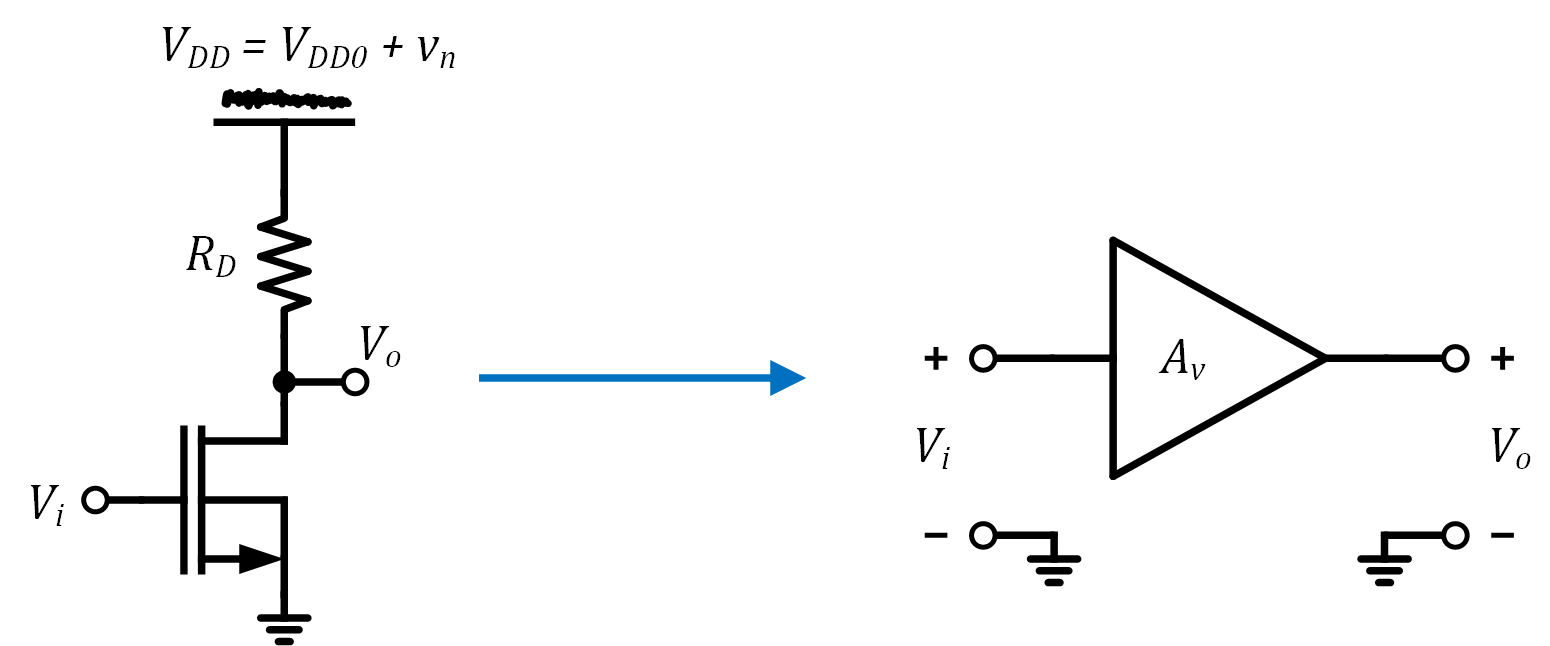
\includegraphics{common_source_single_ended.png}
\caption{common\_source\_single\_ended.png}
\end{figure}

    \begin{itemize}
\item
  ``Single-ended'' circuits are those whose inputs/outputs are
  referenced to a \(DC\) voltage (usually \(V_{DD}\) or \(GND\))
\item
  Supply voltages are not ideal \(DC\) voltages, but have time-varying
  content in the form of noise/disturbances
  (i.e.~\(V_{DD} = V_{DD0} + v_n\))
\item
  As a result, the signal voltage can easily be corrupted by noise on
  the reference (e.g.~\(GND\))
\end{itemize}

    \begin{itemize}
\tightlist
\item
  In the case of a resistively-loaded commmon-source amplifier, supply
  noise adds directly to the amplifier output:
\end{itemize}

\begin{align}
V_{o} &= V_{DD} - I_D\cdot R_D - 0V + v_{n,gnd}\\
\\
&= V_{DD0} + v_{n,vdd} - (I_{DC} + g_m v_i)R_D + v_{n,gnd}
\end{align}

\begin{itemize}
\tightlist
\item
  The signal voltage is thus
\end{itemize}

\begin{equation}
v_o = -g_m\cdot v_i R_D + v_{n,vdd} + v_{n,gnd}
\end{equation}

\begin{itemize}
\tightlist
\item
  How can we mitigate this?
\end{itemize}

    \hypertarget{differential-amplifiers}{%
\subsection{Differential amplifiers}\label{differential-amplifiers}}

    \begin{figure}
\centering
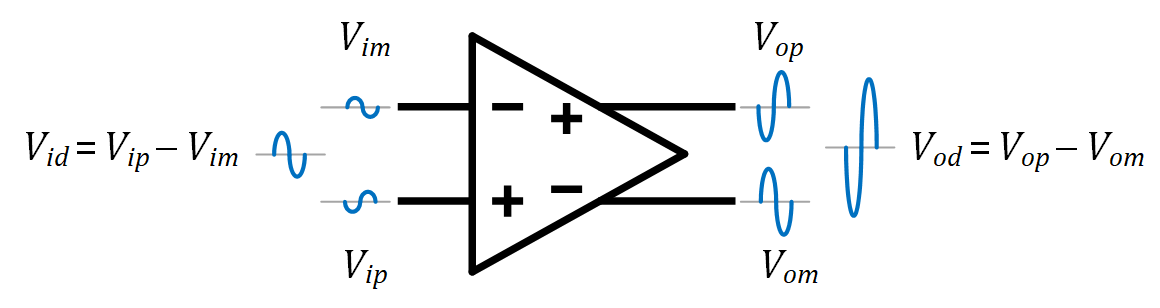
\includegraphics{differential_signaling.png}
\caption{differential\_signaling.png}
\end{figure}

    \begin{itemize}
\tightlist
\item
  Differential amplifiers operate with \emph{differential} input and
  output signals
\item
  Differential signals comprise the \emph{differences} between
  differential voltage pairs
\item
  Because they are \(180^\circ\) out of phase with each other, the
  amplitudes of differential signals (\(V_{id}\), \(V_{od}\)) are twice
  that of the individual voltages
\end{itemize}

    \hypertarget{differential-vs-common-mode}{%
\subsection{Differential vs
common-mode}\label{differential-vs-common-mode}}

    \begin{figure}
\centering
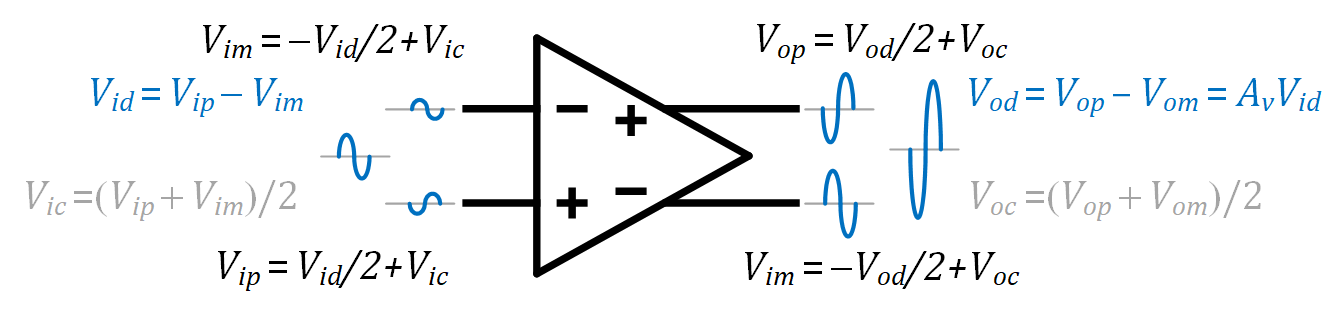
\includegraphics{DM_vs_CM.png}
\caption{DM\_vs\_CM.png}
\end{figure}

    \begin{itemize}
\tightlist
\item
  Each input or output voltage consists of a common-mode and a
  differential-mode component
\item
  The differential-mode voltages at the input (\(V_{id}\)) and output
  (\(V_{od}\)) are related through the voltage gain of the amplifier
  (\(A_v\))
\item
  The common-mode voltages at the input (\(V_{ic}\)) and output
  (\(V_{oc}\)) are (ideally) independent of each other
\item
  In this sense, common-mode signals are suppressed, while differential
  signals are amplified
\end{itemize}

    \hypertarget{differential-signal-common-mode-noise}{%
\subsection{Differential signal, common-mode
noise}\label{differential-signal-common-mode-noise}}

    \begin{itemize}
\tightlist
\item
  Let's take a look at an example of differential versus common-mode
  signal components
\end{itemize}

    \begin{tcolorbox}[breakable, size=fbox, boxrule=1pt, pad at break*=1mm,colback=cellbackground, colframe=cellborder]
\prompt{In}{incolor}{36}{\boxspacing}
\begin{Verbatim}[commandchars=\\\{\}]
\PY{c+c1}{\PYZsh{} Define a sinusoidal signal with DC level}
\PY{n}{f} \PY{o}{=} \PY{l+m+mf}{1e3}
\PY{n}{w} \PY{o}{=} \PY{n}{f}\PY{o}{*}\PY{l+m+mi}{2}\PY{o}{*}\PY{n}{np}\PY{o}{.}\PY{n}{pi}
\PY{n}{t} \PY{o}{=} \PY{n}{np}\PY{o}{.}\PY{n}{linspace}\PY{p}{(}\PY{l+m+mi}{0}\PY{p}{,}\PY{l+m+mf}{3e\PYZhy{}3}\PY{p}{,}\PY{n}{num}\PY{o}{=}\PY{l+m+mi}{300}\PY{p}{)}
\PY{n}{V\PYZus{}dd} \PY{o}{=} \PY{l+m+mf}{3.3}
\PY{n}{V\PYZus{}cm} \PY{o}{=} \PY{n}{V\PYZus{}dd}\PY{o}{/}\PY{l+m+mi}{2} 
\PY{n}{v\PYZus{}plus} \PY{o}{=} \PY{n}{V\PYZus{}cm} \PY{o}{+} \PY{l+m+mf}{1e\PYZhy{}3}\PY{o}{*}\PY{n}{np}\PY{o}{.}\PY{n}{sin}\PY{p}{(}\PY{n}{w}\PY{o}{*}\PY{n}{t}\PY{p}{)}
\PY{n}{v\PYZus{}minus} \PY{o}{=} \PY{n}{V\PYZus{}cm} \PY{o}{\PYZhy{}} \PY{l+m+mf}{1e\PYZhy{}3}\PY{o}{*}\PY{n}{np}\PY{o}{.}\PY{n}{sin}\PY{p}{(}\PY{n}{w}\PY{o}{*}\PY{n}{t}\PY{p}{)}

\PY{c+c1}{\PYZsh{} Define a random noise source}
\PY{n}{mu} \PY{o}{=} \PY{l+m+mi}{0}
\PY{n}{sigma} \PY{o}{=} \PY{l+m+mf}{100e\PYZhy{}6}
\PY{n}{v\PYZus{}noise} \PY{o}{=} \PY{n}{np}\PY{o}{.}\PY{n}{random}\PY{o}{.}\PY{n}{normal}\PY{p}{(}\PY{n}{mu}\PY{p}{,} \PY{n}{sigma}\PY{p}{,} \PY{l+m+mi}{300}\PY{p}{)}

\PY{c+c1}{\PYZsh{} Combine the two}
\PY{n}{vd\PYZus{}plus} \PY{o}{=} \PY{n}{v\PYZus{}plus} \PY{o}{+} \PY{n}{v\PYZus{}noise}
\PY{n}{vd\PYZus{}minus} \PY{o}{=} \PY{n}{v\PYZus{}minus} \PY{o}{+} \PY{n}{v\PYZus{}noise}
\PY{n}{v\PYZus{}diff} \PY{o}{=} \PY{n}{vd\PYZus{}plus} \PY{o}{\PYZhy{}} \PY{n}{vd\PYZus{}minus}
\end{Verbatim}
\end{tcolorbox}

    \begin{tcolorbox}[breakable, size=fbox, boxrule=1pt, pad at break*=1mm,colback=cellbackground, colframe=cellborder]
\prompt{In}{incolor}{37}{\boxspacing}
\begin{Verbatim}[commandchars=\\\{\}]
\PY{n}{plot\PYZus{}xy3}\PY{p}{(}\PY{l+m+mf}{1e3}\PY{o}{*}\PY{n}{t}\PY{p}{,} \PY{n}{vd\PYZus{}plus}\PY{p}{,} \PY{n}{vd\PYZus{}minus}\PY{p}{,} \PY{l+m+mf}{1e3}\PY{o}{*}\PY{n}{v\PYZus{}diff}\PY{p}{,}
        \PY{l+s+s1}{\PYZsq{}}\PY{l+s+s1}{Time [ms]}\PY{l+s+s1}{\PYZsq{}}\PY{p}{,}\PY{l+s+s1}{\PYZsq{}}\PY{l+s+s1}{\PYZdl{}v\PYZus{}+\PYZdl{} [V]}\PY{l+s+s1}{\PYZsq{}}\PY{p}{,}\PY{l+s+s1}{\PYZsq{}}\PY{l+s+s1}{\PYZdl{}v\PYZus{}\PYZhy{}\PYZdl{} [V]}\PY{l+s+s1}{\PYZsq{}}\PY{p}{,}\PY{l+s+s1}{\PYZsq{}}\PY{l+s+s1}{\PYZdl{}v\PYZus{}+ \PYZhy{} v\PYZus{}\PYZhy{}\PYZdl{} [mV]}\PY{l+s+s1}{\PYZsq{}}\PY{p}{)}
\end{Verbatim}
\end{tcolorbox}

    \begin{center}
    \adjustimage{max size={0.9\linewidth}{0.9\paperheight}}{2021_02_03_EE538_Lecture5_W2021_files/2021_02_03_EE538_Lecture5_W2021_23_0.png}
    \end{center}
    { \hspace*{\fill} \\}
    
    \begin{itemize}
\tightlist
\item
  Differential processing suppresses noise due to a circuit property
  referred to as \emph{common-mode rejection}
\item
  In this case, the common-mode rejection is perfect (i.e.~infinite), as
  it is based on arithmetic subtraction
\item
  Note that many types of noise are \emph{not} common-mode (e.g.~thermal
  noise), and are thus not removed by differential signaling
\end{itemize}

    \hypertarget{snr-advantage}{%
\subsection{SNR advantage}\label{snr-advantage}}

    \begin{figure}
\centering
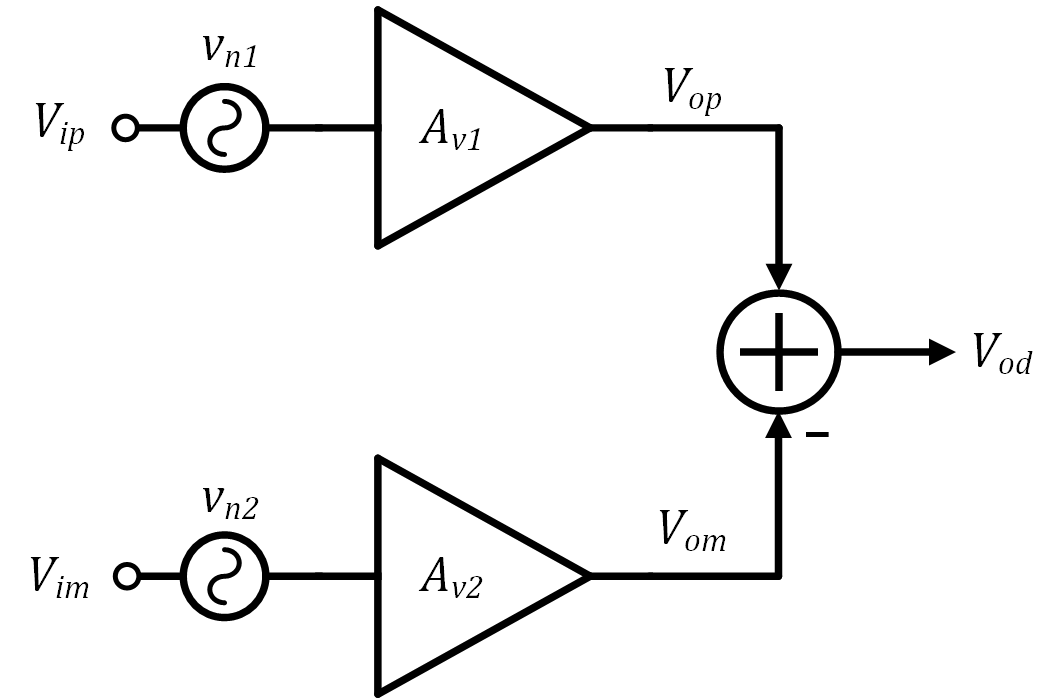
\includegraphics{differential_noise.png}
\caption{differential\_noise.png}
\end{figure}

    \begin{itemize}
\tightlist
\item
  All electronic circuits generate thermal noise that corrupts signals
  and degrades signal-to-noise ratio (SNR)
\item
  Differential signaling allows us to take advantage of the fact that
  independent noise processes are uncorrelated
\item
  Uncorrelated noise sources (\(v_{n1}\) and \(v_{n2}\)) add in a
  \emph{mean-square} sense, while differential signals (\(V_{ip}\) and
  \(V_{im}\)) are correlated and add directly
\end{itemize}

    \begin{itemize}
\tightlist
\item
  For example, \(v_{n1}\) and \(v_{n2}\) represent the
  \emph{input-referred} noise of \(A_{v1}\) and \(A_{v2}\), respectively
\end{itemize}

    \begin{tcolorbox}[breakable, size=fbox, boxrule=1pt, pad at break*=1mm,colback=cellbackground, colframe=cellborder]
\prompt{In}{incolor}{38}{\boxspacing}
\begin{Verbatim}[commandchars=\\\{\}]
\PY{c+c1}{\PYZsh{} Define a sinusoidal signal with DC level}
\PY{n}{f} \PY{o}{=} \PY{l+m+mf}{1e3}
\PY{n}{w} \PY{o}{=} \PY{n}{f}\PY{o}{*}\PY{l+m+mi}{2}\PY{o}{*}\PY{n}{np}\PY{o}{.}\PY{n}{pi}
\PY{n}{t} \PY{o}{=} \PY{n}{np}\PY{o}{.}\PY{n}{linspace}\PY{p}{(}\PY{l+m+mi}{0}\PY{p}{,}\PY{l+m+mf}{20e\PYZhy{}3}\PY{p}{,}\PY{n}{num}\PY{o}{=}\PY{l+m+mi}{1000}\PY{p}{)}
\PY{n}{V\PYZus{}cm} \PY{o}{=} \PY{l+m+mi}{0}
\PY{n}{A\PYZus{}v1} \PY{o}{=} \PY{l+m+mi}{1}
\PY{n}{A\PYZus{}v2} \PY{o}{=} \PY{l+m+mi}{1}
\PY{n}{v\PYZus{}ip} \PY{o}{=} \PY{n}{V\PYZus{}cm} \PY{o}{+} \PY{l+m+mf}{1e\PYZhy{}3}\PY{o}{*}\PY{n}{np}\PY{o}{.}\PY{n}{sin}\PY{p}{(}\PY{n}{w}\PY{o}{*}\PY{n}{t}\PY{p}{)}
\PY{n}{v\PYZus{}im} \PY{o}{=} \PY{n}{V\PYZus{}cm} \PY{o}{\PYZhy{}} \PY{l+m+mf}{1e\PYZhy{}3}\PY{o}{*}\PY{n}{np}\PY{o}{.}\PY{n}{sin}\PY{p}{(}\PY{n}{w}\PY{o}{*}\PY{n}{t}\PY{p}{)}

\PY{c+c1}{\PYZsh{} Define a random noise source}
\PY{n}{mu} \PY{o}{=} \PY{l+m+mi}{0}
\PY{n}{sigma} \PY{o}{=} \PY{l+m+mf}{100e\PYZhy{}6}
\PY{n}{v\PYZus{}n1} \PY{o}{=} \PY{n}{np}\PY{o}{.}\PY{n}{random}\PY{o}{.}\PY{n}{normal}\PY{p}{(}\PY{n}{mu}\PY{p}{,} \PY{n}{sigma}\PY{p}{,} \PY{l+m+mi}{1000}\PY{p}{)}
\PY{n}{v\PYZus{}n2} \PY{o}{=} \PY{n}{np}\PY{o}{.}\PY{n}{random}\PY{o}{.}\PY{n}{normal}\PY{p}{(}\PY{n}{mu}\PY{p}{,} \PY{n}{sigma}\PY{p}{,} \PY{l+m+mi}{1000}\PY{p}{)}

\PY{c+c1}{\PYZsh{} Combine the two}
\PY{n}{v\PYZus{}op} \PY{o}{=} \PY{n}{A\PYZus{}v1}\PY{o}{*}\PY{p}{(}\PY{n}{v\PYZus{}ip} \PY{o}{+} \PY{n}{v\PYZus{}n1}\PY{p}{)}
\PY{n}{v\PYZus{}om} \PY{o}{=} \PY{n}{A\PYZus{}v2}\PY{o}{*}\PY{p}{(}\PY{n}{v\PYZus{}im} \PY{o}{+} \PY{n}{v\PYZus{}n2}\PY{p}{)}
\PY{n}{v\PYZus{}od} \PY{o}{=} \PY{n}{v\PYZus{}op} \PY{o}{\PYZhy{}} \PY{n}{v\PYZus{}om}
\end{Verbatim}
\end{tcolorbox}

    \begin{tcolorbox}[breakable, size=fbox, boxrule=1pt, pad at break*=1mm,colback=cellbackground, colframe=cellborder]
\prompt{In}{incolor}{39}{\boxspacing}
\begin{Verbatim}[commandchars=\\\{\}]
\PY{n}{plot\PYZus{}xy3}\PY{p}{(}\PY{l+m+mf}{1e3}\PY{o}{*}\PY{n}{t}\PY{p}{,} \PY{n}{v\PYZus{}op}\PY{p}{,} \PY{n}{v\PYZus{}om}\PY{p}{,} \PY{l+m+mf}{1e3}\PY{o}{*}\PY{n}{v\PYZus{}od}\PY{p}{,}
        \PY{l+s+s1}{\PYZsq{}}\PY{l+s+s1}{Time [ms]}\PY{l+s+s1}{\PYZsq{}}\PY{p}{,}\PY{l+s+s1}{\PYZsq{}}\PY{l+s+s1}{\PYZdl{}v\PYZus{}+\PYZdl{} [V]}\PY{l+s+s1}{\PYZsq{}}\PY{p}{,}\PY{l+s+s1}{\PYZsq{}}\PY{l+s+s1}{\PYZdl{}v\PYZus{}\PYZhy{}\PYZdl{} [V]}\PY{l+s+s1}{\PYZsq{}}\PY{p}{,}\PY{l+s+s1}{\PYZsq{}}\PY{l+s+s1}{\PYZdl{}v\PYZus{}+ \PYZhy{} v\PYZus{}\PYZhy{}\PYZdl{} [mV]}\PY{l+s+s1}{\PYZsq{}}\PY{p}{)}
\end{Verbatim}
\end{tcolorbox}

    \begin{center}
    \adjustimage{max size={0.9\linewidth}{0.9\paperheight}}{2021_02_03_EE538_Lecture5_W2021_files/2021_02_03_EE538_Lecture5_W2021_30_0.png}
    \end{center}
    { \hspace*{\fill} \\}
    
    \begin{itemize}
\tightlist
\item
  To understand the the noise advantage offered by differential
  signaling, we need to compare the SNR of the individual amplifier
  outputs with that of the differential signal
\end{itemize}

    \begin{tcolorbox}[breakable, size=fbox, boxrule=1pt, pad at break*=1mm,colback=cellbackground, colframe=cellborder]
\prompt{In}{incolor}{40}{\boxspacing}
\begin{Verbatim}[commandchars=\\\{\}]
\PY{n}{snr1} \PY{o}{=} \PY{n}{np}\PY{o}{.}\PY{n}{std}\PY{p}{(}\PY{n}{A\PYZus{}v1}\PY{o}{*}\PY{n}{v\PYZus{}op}\PY{p}{)}\PY{o}{/}\PY{n}{np}\PY{o}{.}\PY{n}{std}\PY{p}{(}\PY{n}{A\PYZus{}v1}\PY{o}{*}\PY{n}{v\PYZus{}n1}\PY{p}{)}
\PY{n}{snr2} \PY{o}{=} \PY{n}{np}\PY{o}{.}\PY{n}{std}\PY{p}{(}\PY{n}{A\PYZus{}v2}\PY{o}{*}\PY{n}{v\PYZus{}om}\PY{p}{)}\PY{o}{/}\PY{n}{np}\PY{o}{.}\PY{n}{std}\PY{p}{(}\PY{n}{A\PYZus{}v2}\PY{o}{*}\PY{n}{v\PYZus{}n2}\PY{p}{)}
\PY{n}{snr\PYZus{}diff} \PY{o}{=} \PY{n}{np}\PY{o}{.}\PY{n}{std}\PY{p}{(}\PY{n}{v\PYZus{}od}\PY{p}{)}\PY{o}{/}\PY{n}{np}\PY{o}{.}\PY{n}{std}\PY{p}{(}\PY{n}{A\PYZus{}v1}\PY{o}{*}\PY{p}{(}\PY{n}{v\PYZus{}n1}\PY{o}{+}\PY{n}{v\PYZus{}n2}\PY{p}{)}\PY{p}{)}
\end{Verbatim}
\end{tcolorbox}

    \begin{itemize}
\tightlist
\item
  The signal-to-noise ratio of the individual outputs are approximately
  equal and given by
\end{itemize}

    \begin{tcolorbox}[breakable, size=fbox, boxrule=1pt, pad at break*=1mm,colback=cellbackground, colframe=cellborder]
\prompt{In}{incolor}{41}{\boxspacing}
\begin{Verbatim}[commandchars=\\\{\}]
\PY{n+nb}{print}\PY{p}{(}\PY{l+s+s1}{\PYZsq{}}\PY{l+s+s1}{The SNR for v\PYZus{}op is}\PY{l+s+s1}{\PYZsq{}}\PY{p}{,} \PY{n}{snr1}\PY{p}{)}
\PY{n+nb}{print}\PY{p}{(}\PY{l+s+s1}{\PYZsq{}}\PY{l+s+s1}{The SNR for v\PYZus{}om is}\PY{l+s+s1}{\PYZsq{}}\PY{p}{,} \PY{n}{snr2}\PY{p}{)}
\end{Verbatim}
\end{tcolorbox}

    \begin{Verbatim}[commandchars=\\\{\}]
The SNR for v\_op is 7.054509679327141
The SNR for v\_om is 7.1293784742064785
    \end{Verbatim}

    \begin{itemize}
\tightlist
\item
  The SNR of the differential output is given by
\end{itemize}

    \begin{tcolorbox}[breakable, size=fbox, boxrule=1pt, pad at break*=1mm,colback=cellbackground, colframe=cellborder]
\prompt{In}{incolor}{42}{\boxspacing}
\begin{Verbatim}[commandchars=\\\{\}]
\PY{n+nb}{print}\PY{p}{(}\PY{l+s+s1}{\PYZsq{}}\PY{l+s+s1}{The SNR for v\PYZus{}od is}\PY{l+s+s1}{\PYZsq{}}\PY{p}{,} \PY{n}{snr\PYZus{}diff}\PY{p}{)}
\end{Verbatim}
\end{tcolorbox}

    \begin{Verbatim}[commandchars=\\\{\}]
The SNR for v\_od is 10.111836903087625
    \end{Verbatim}

    \begin{itemize}
\tightlist
\item
  The differential signal amplitude is twice that of the individual
  amplifier outputs while the total noise is only \(\sqrt{2}\) times
  higher, increasing SNR by a factor of \(\sqrt{2}\)
\end{itemize}

    \hypertarget{basic-differential-pair}{%
\subsection{Basic differential pair}\label{basic-differential-pair}}

    \begin{figure}
\centering
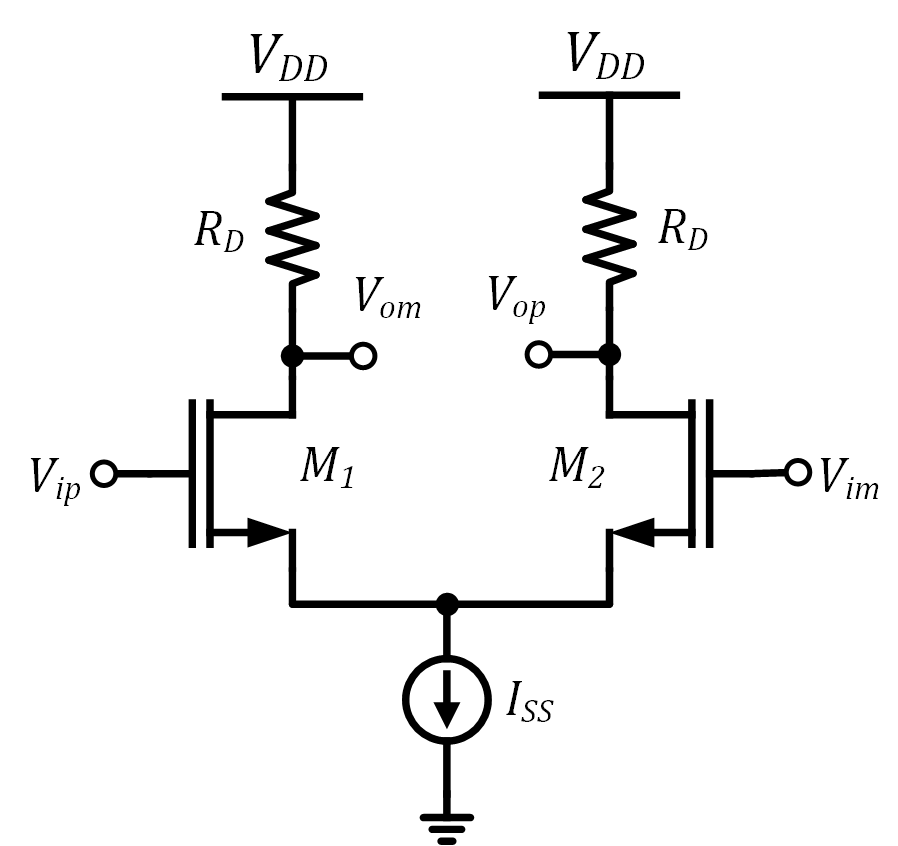
\includegraphics{diff_pair_Rload.png}
\caption{diff\_pair\_Rload.png}
\end{figure}

    \begin{itemize}
\item
  When \(V_{ip} = V_{im}\),
  \(I_{D1} = I_{D2} = \frac{1}{2} \cdot I_{SS}\)
\item
  The output bias (\(DC\) operating) point is set by the product of
  \(I_{SS}\) and \(R_D\)
\item
  As \(V_{id}\) changes from very negative to very positive values, the
  bias current \(I_{SS}\) is ``steered'' from \(M_2\) to \(M_1\)
\item
  \(V_{op}\) goes from \(V_{DD} – I_{SS} \cdot R_D\) to \(V_{DD}\)
  (\(V_{om}\) does the opposite)
\item
  Gain is determined by \(I_{SS}\) and sizing of \(M_{1,2}\)
  (current-biased circuit)
\item
  Gain magnitude is identical to that of a common source with a
  resistive load
\end{itemize}

    \hypertarget{large-signal-operation}{%
\subsection{Large-signal operation}\label{large-signal-operation}}

    \begin{itemize}
\tightlist
\item
  When \(M_1\) (\(M_2\)) is in saturation, drain currents are given by
\end{itemize}

\begin{equation}
I_{d1,2} = \dfrac{I_{SS}}{2} \pm \dfrac{\mu C_{ox}}{4}\dfrac{W}{L}(V_{ip}-V_{im})\sqrt{\dfrac{4I_{SS}}{\mu C_{ox} (W/L)} - (V_{ip} - V_{im})^2}
\end{equation}

\begin{itemize}
\tightlist
\item
  The ouput voltages are then
\end{itemize}

\begin{align}
V_{op} &= V_{DD} - I_{d1}R_D\\
V_{om} &= V_{DD} - I_{d2}R_D
\end{align}

\begin{itemize}
\tightlist
\item
  The differential voltage is their difference:
\end{itemize}

\begin{equation}
V_{od} = V_{op} - V_{om}
\end{equation}

    \begin{tcolorbox}[breakable, size=fbox, boxrule=1pt, pad at break*=1mm,colback=cellbackground, colframe=cellborder]
\prompt{In}{incolor}{83}{\boxspacing}
\begin{Verbatim}[commandchars=\\\{\}]
\PY{n}{V\PYZus{}dd} \PY{o}{=} \PY{l+m+mi}{3}
\PY{n}{R\PYZus{}D} \PY{o}{=} \PY{l+m+mf}{1e3}
\PY{n}{I\PYZus{}SS} \PY{o}{=} \PY{l+m+mf}{1e\PYZhy{}3}
\PY{n}{V\PYZus{}id} \PY{o}{=} \PY{n}{np}\PY{o}{.}\PY{n}{arange}\PY{p}{(}\PY{o}{\PYZhy{}}\PY{l+m+mf}{1.2}\PY{p}{,} \PY{l+m+mf}{1.2}\PY{p}{,} \PY{n}{step}\PY{o}{=}\PY{l+m+mf}{0.01}\PY{p}{)}
\PY{n}{I\PYZus{}d1}\PY{p}{,} \PY{n}{I\PYZus{}d2} \PY{o}{=} \PY{n}{nmos\PYZus{}diff\PYZus{}pair}\PY{p}{(}\PY{n}{V\PYZus{}id}\PY{p}{,} \PY{n}{I\PYZus{}SS}\PY{p}{,} \PY{n}{R\PYZus{}D}\PY{p}{,} \PY{l+m+mi}{10}\PY{p}{,} \PY{l+m+mi}{1}\PY{p}{,} \PY{n}{V\PYZus{}dd}\PY{p}{)}

\PY{n}{plot\PYZus{}x2y}\PY{p}{(}\PY{n}{V\PYZus{}id}\PY{p}{,} \PY{l+m+mf}{1e3}\PY{o}{*}\PY{n}{I\PYZus{}d1}\PY{p}{,} \PY{l+m+mf}{1e3}\PY{o}{*}\PY{n}{I\PYZus{}d2}\PY{p}{,} \PY{l+s+sa}{r}\PY{l+s+s1}{\PYZsq{}}\PY{l+s+s1}{\PYZdl{}V\PYZus{}}\PY{l+s+si}{\PYZob{}id\PYZcb{}}\PY{l+s+s1}{\PYZdl{}}\PY{l+s+s1}{\PYZsq{}}\PY{p}{,} \PY{l+s+s1}{\PYZsq{}}\PY{l+s+s1}{Drain Current [mA]}\PY{l+s+s1}{\PYZsq{}}\PY{p}{,} \PY{l+s+sa}{r}\PY{l+s+s1}{\PYZsq{}}\PY{l+s+s1}{\PYZdl{}I\PYZus{}}\PY{l+s+si}{\PYZob{}d1\PYZcb{}}\PY{l+s+s1}{\PYZdl{}}\PY{l+s+s1}{\PYZsq{}}\PY{p}{,} \PY{l+s+sa}{r}\PY{l+s+s1}{\PYZsq{}}\PY{l+s+s1}{\PYZdl{}I\PYZus{}}\PY{l+s+si}{\PYZob{}d2\PYZcb{}}\PY{l+s+s1}{\PYZdl{}}\PY{l+s+s1}{\PYZsq{}}\PY{p}{)}
\end{Verbatim}
\end{tcolorbox}

    \begin{center}
    \adjustimage{max size={0.9\linewidth}{0.9\paperheight}}{2021_02_03_EE538_Lecture5_W2021_files/2021_02_03_EE538_Lecture5_W2021_43_0.png}
    \end{center}
    { \hspace*{\fill} \\}
    
    \begin{tcolorbox}[breakable, size=fbox, boxrule=1pt, pad at break*=1mm,colback=cellbackground, colframe=cellborder]
\prompt{In}{incolor}{84}{\boxspacing}
\begin{Verbatim}[commandchars=\\\{\}]
\PY{n}{V\PYZus{}op} \PY{o}{=} \PY{n}{V\PYZus{}dd} \PY{o}{\PYZhy{}} \PY{n}{I\PYZus{}d1}\PY{o}{*}\PY{n}{R\PYZus{}D}
\PY{n}{V\PYZus{}om} \PY{o}{=} \PY{n}{V\PYZus{}dd} \PY{o}{\PYZhy{}} \PY{n}{I\PYZus{}d2}\PY{o}{*}\PY{n}{R\PYZus{}D}
\PY{n}{plot\PYZus{}x2y}\PY{p}{(}\PY{n}{V\PYZus{}id}\PY{p}{,} \PY{n}{V\PYZus{}op}\PY{p}{,} \PY{n}{V\PYZus{}om}\PY{p}{,} \PY{l+s+sa}{r}\PY{l+s+s1}{\PYZsq{}}\PY{l+s+s1}{\PYZdl{}V\PYZus{}}\PY{l+s+si}{\PYZob{}id\PYZcb{}}\PY{l+s+s1}{\PYZdl{}}\PY{l+s+s1}{\PYZsq{}}\PY{p}{,} \PY{l+s+s1}{\PYZsq{}}\PY{l+s+s1}{Output Voltage [V]}\PY{l+s+s1}{\PYZsq{}}\PY{p}{,} \PY{l+s+sa}{r}\PY{l+s+s1}{\PYZsq{}}\PY{l+s+s1}{\PYZdl{}V\PYZus{}}\PY{l+s+si}{\PYZob{}op\PYZcb{}}\PY{l+s+s1}{\PYZdl{}}\PY{l+s+s1}{\PYZsq{}}\PY{p}{,} \PY{l+s+sa}{r}\PY{l+s+s1}{\PYZsq{}}\PY{l+s+s1}{\PYZdl{}V\PYZus{}}\PY{l+s+si}{\PYZob{}om\PYZcb{}}\PY{l+s+s1}{\PYZdl{}}\PY{l+s+s1}{\PYZsq{}}\PY{p}{)}
\end{Verbatim}
\end{tcolorbox}

    \begin{center}
    \adjustimage{max size={0.9\linewidth}{0.9\paperheight}}{2021_02_03_EE538_Lecture5_W2021_files/2021_02_03_EE538_Lecture5_W2021_44_0.png}
    \end{center}
    { \hspace*{\fill} \\}
    
    \begin{itemize}
\tightlist
\item
  For \(V_{ip}\) (\(V_{im}\)) less than \(V_{th}\), \(M_1\) (\(M_2\)) is
  off and \(V_{om}\) (\(V_{op}\)) is at \(V_{DD}\)
\item
  For \(V_{ip}\) (\(V_{im}\)) \(\approx V_{DD}\), \(M_1\) (\(M_2\)) is
  in triode
\item
  Gain is at its maximum value for \(V_{id} = 0\)
\end{itemize}

    \hypertarget{small-signal-model}{%
\subsection{Small-signal model}\label{small-signal-model}}

    \begin{figure}
\centering
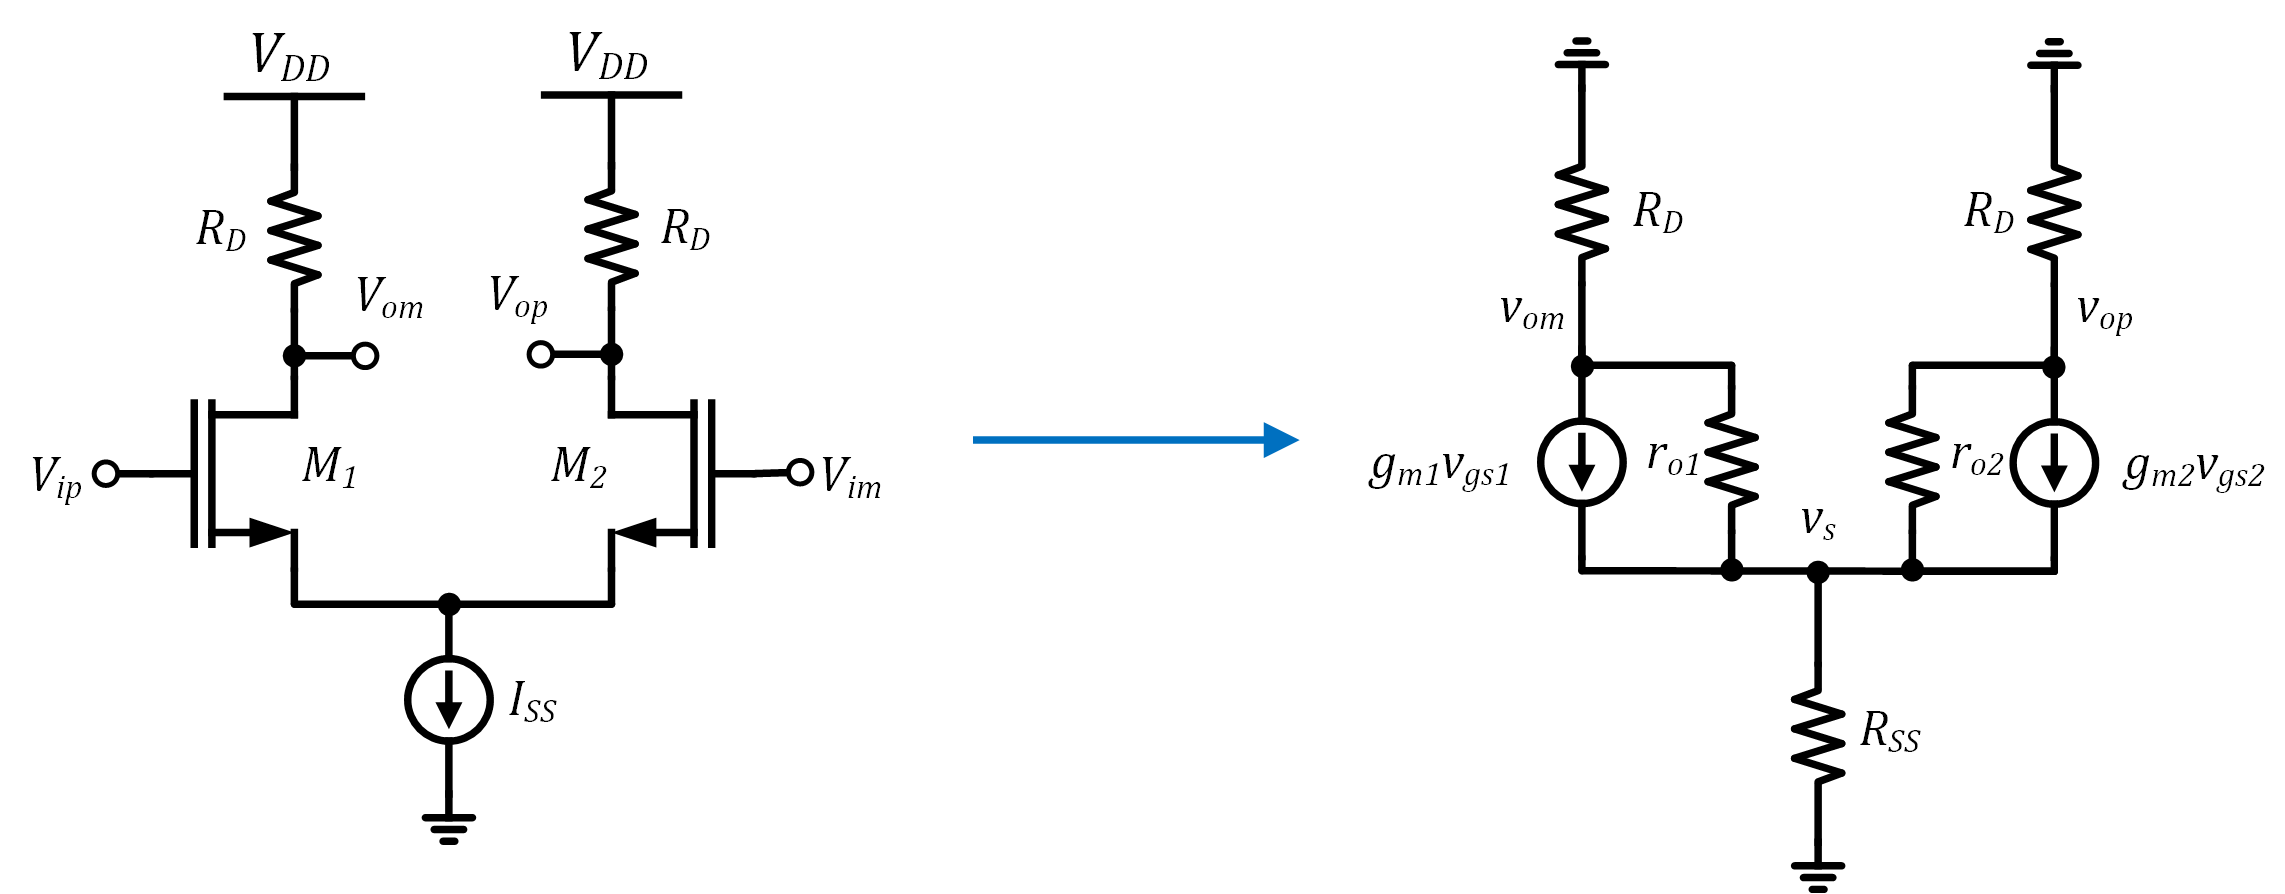
\includegraphics{diff_pair_small_signal.png}
\caption{diff\_pair\_small\_signal.png}
\end{figure}

    \begin{itemize}
\tightlist
\item
  \(M_1\) and \(M_2\) ared designed to be identical,
  i.e.~\((W/L)_1 = (W/L)_2\)
\item
  For \(V_{ip} = V_{im}\) (\(V_{id} = 0\)), \(I_{D1} = I_{D2}\), so
  \(g_{m1} = g_{m2}\)
\item
  \(R_{SS}\) represents the output resistance of a current source
  (e.g.~MOS \(r_o\) or cascode \(R_o\))
\item
  Body effect has been ignored for simplicity, but will typically be
  present for \(M_{1,2}\)
\end{itemize}

    \hypertarget{differential-mode-operation}{%
\subsection{Differential-mode
operation}\label{differential-mode-operation}}

    \begin{figure}
\centering
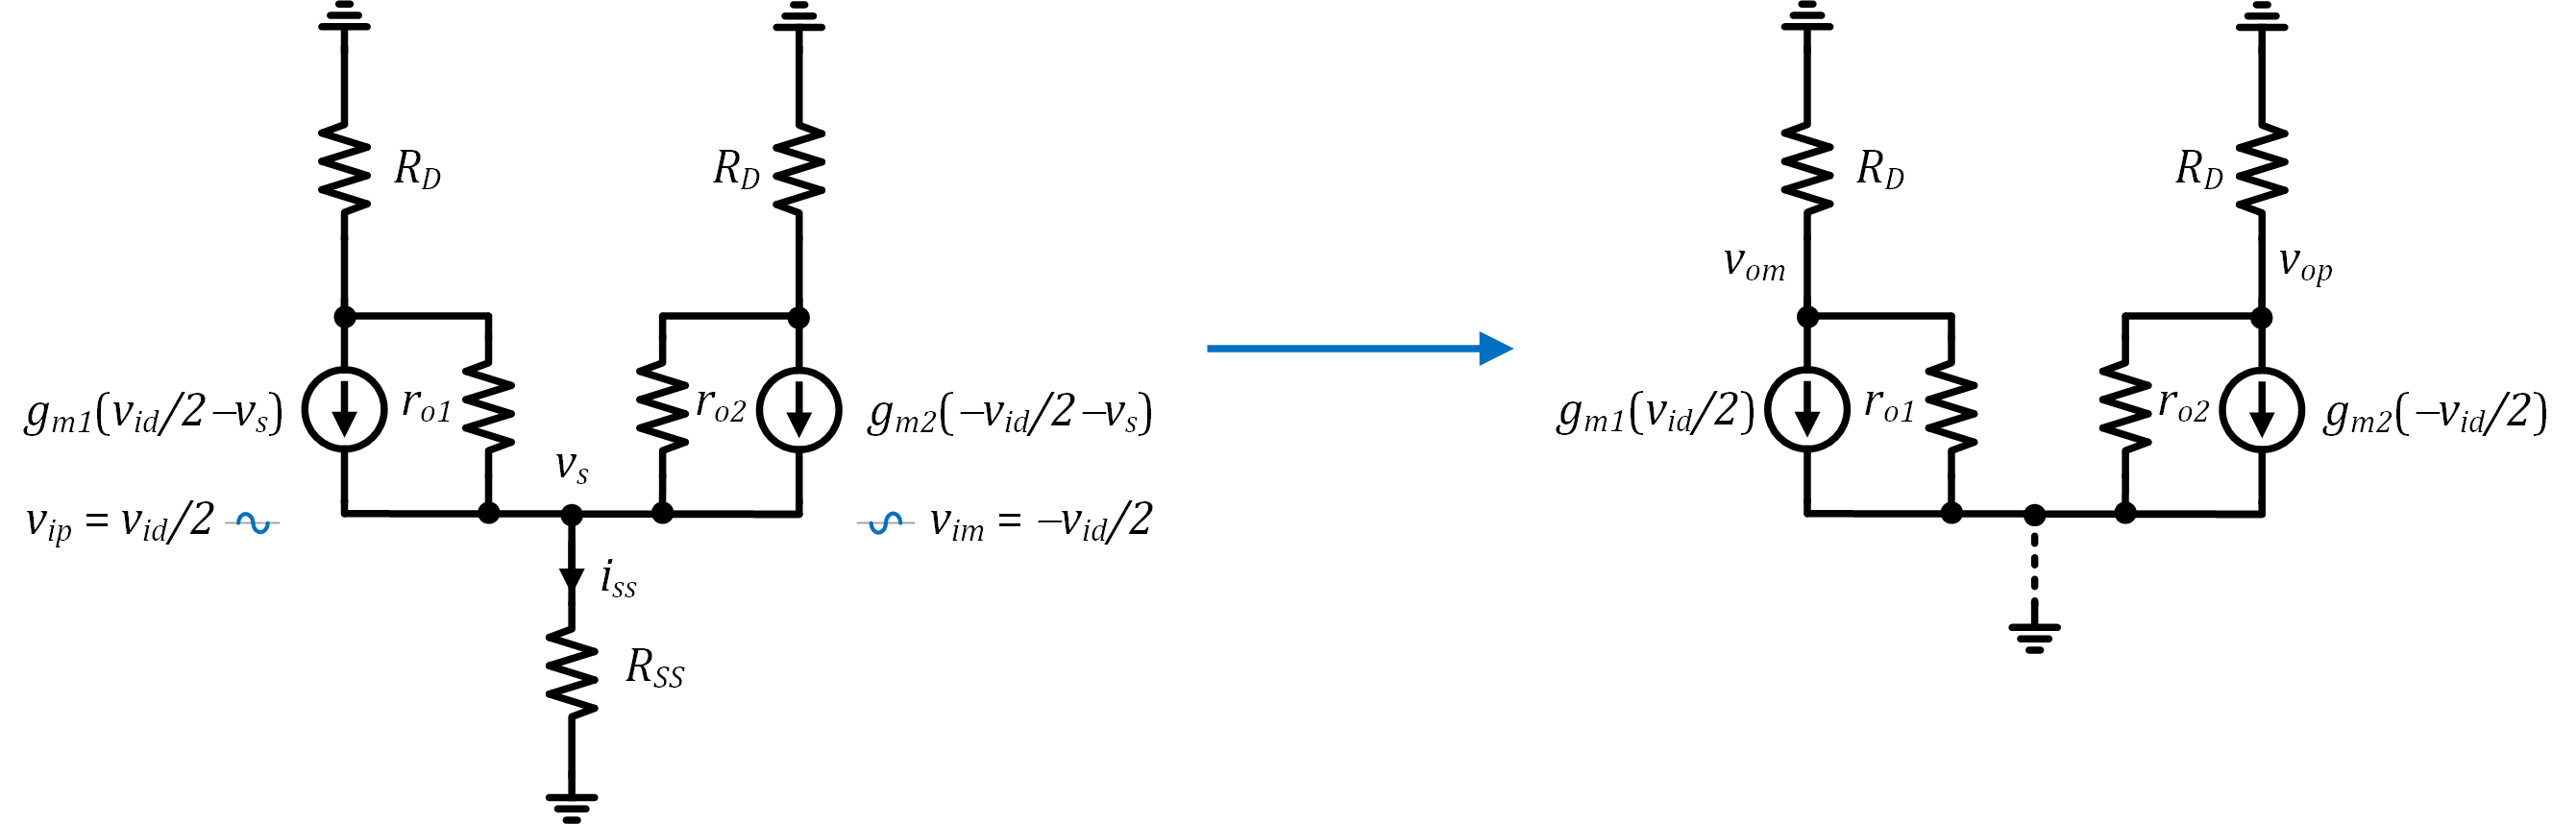
\includegraphics{diff_amp_small_signal.png}
\caption{diff\_amp\_small\_signal.png}
\end{figure}

    \begin{itemize}
\tightlist
\item
  Because \(g_{m1} = g_{m2}\), the small-signal currents
  \(g_{m1}v_{gs1}\) and \(g_{m2}v_{gs2}\) are \emph{equal in magnitude}
  and \emph{opposite in polarity} for differential inputs
\item
  Ignoring finite \(r_o\), this means that the \emph{net} small-signal
  current \(i_{ss}\) is \(0\)
\item
  Because \(i_{ss} = 0\), \(v_{ss} = 0\), causing \(v_s\) to act as a
  ``virtual'' ground
\end{itemize}

    \hypertarget{differential-mode-gain}{%
\subsection{Differential-mode gain}\label{differential-mode-gain}}

    \begin{figure}
\centering
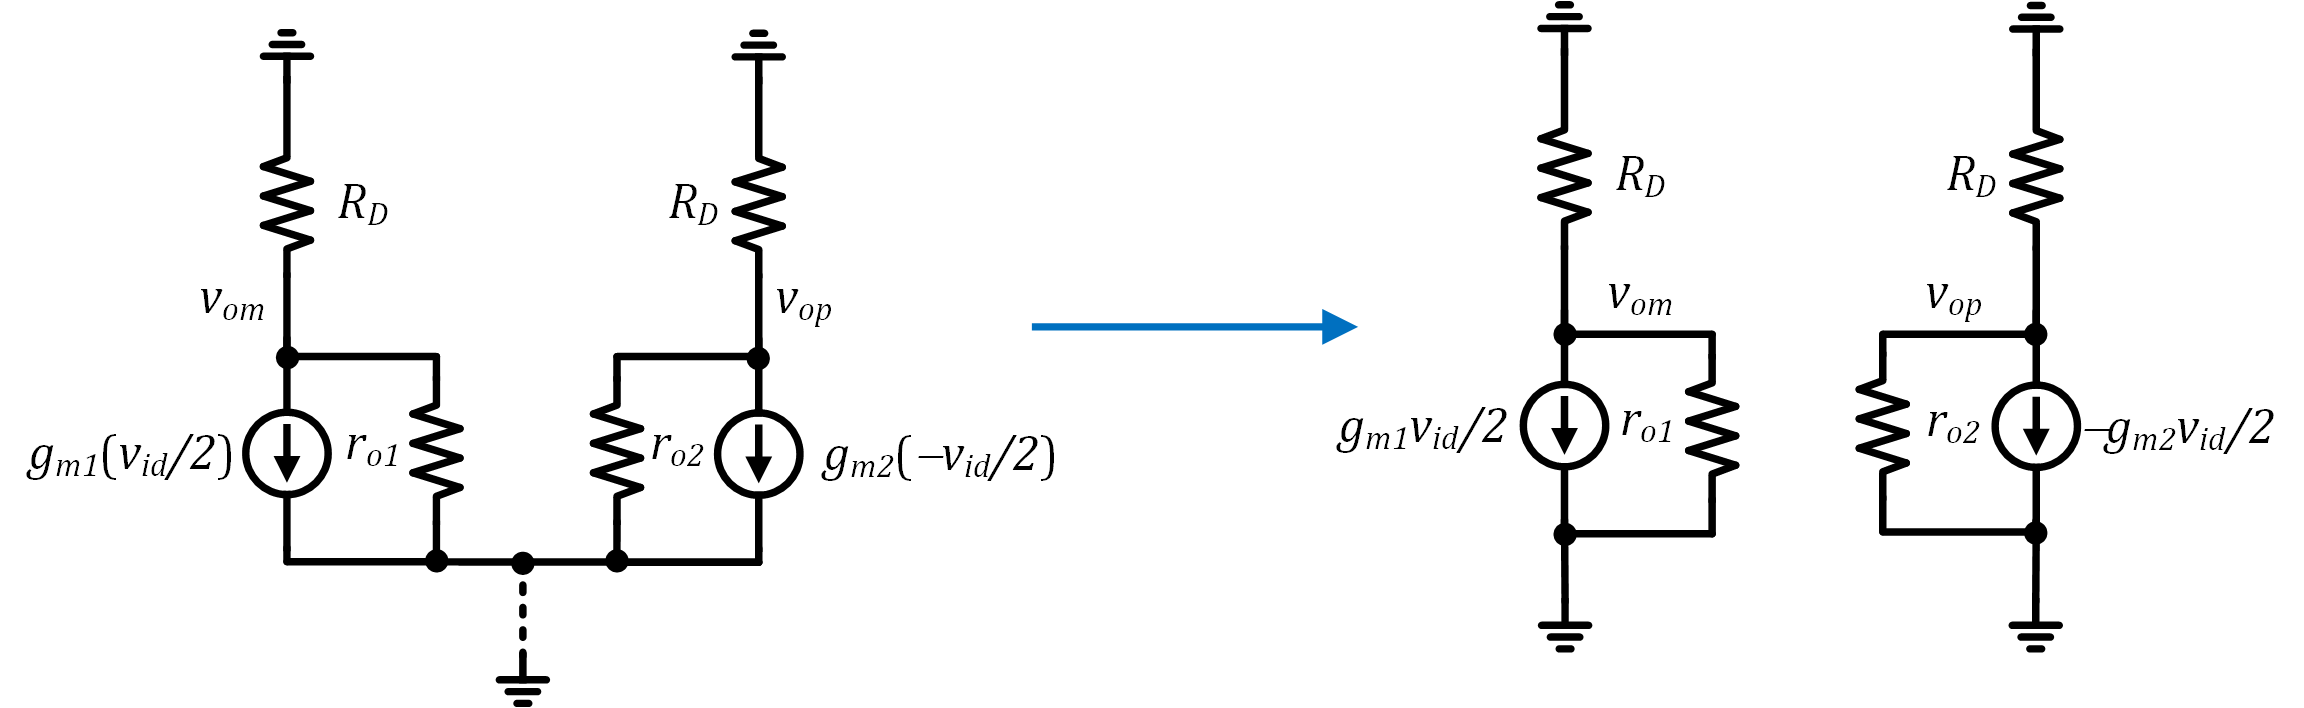
\includegraphics{DM_half_circuit.png}
\caption{DM\_half\_circuit.png}
\end{figure}

    \begin{itemize}
\tightlist
\item
  Due to the virtual ground, the ``half circuit,'' which is symmetric
  for \(v_{ip}\) and \(v_{im}\), can be used for small-signal analysis
\item
  Each half-circuit constitutes a common-source amplifier, and can be
  analyzed separately
\item
  The differential gain is determined by taking the ratio of the
  \emph{difference} of the output voltages to that of the input voltages
\end{itemize}

    \begin{itemize}
\tightlist
\item
  For \(v_{om}\), we have
\end{itemize}

\begin{equation}
v_{om} = -g_{m1}\dfrac{v_{id}}{2}\cdot R_D||r_{o1} \approx -g_{m1}\dfrac{v_{id}}{2}\cdot R_D
\end{equation}

\begin{itemize}
\tightlist
\item
  Similarly, for \(v_{op}\),
\end{itemize}

\begin{equation}
v_{op} \approx g_{m2}\dfrac{v_{id}}{2}\cdot R_D
\end{equation}

\begin{itemize}
\tightlist
\item
  The differential gain is thus
\end{itemize}

\begin{equation}
A_{v,d} = \dfrac{v_{od}}{v_{id}} = \dfrac{v_{op} - v_{om}}{v_{id}} = \dfrac{g_{m2}\cdot \frac{v_{id}}{2}\cdot R_D + g_{m1}\cdot \frac{v_{id}}{2}\cdot R_D}{v_{id}}
\end{equation}

\begin{itemize}
\tightlist
\item
  Since \(g_{m1} = g_{m2} = g_m\), we can write
\end{itemize}

\begin{equation}
A_{v,d} = \dfrac{g_{m}\cdot \frac{v_{id}}{2}\cdot R_D + g_{m} \cdot \frac{v_{id}}{2}\cdot R_D}{v_{id}} = \boxed{g_m\cdot R_D}
\end{equation}

    \hypertarget{common-mode-operation}{%
\subsection{Common-mode operation}\label{common-mode-operation}}

    \begin{figure}
\centering
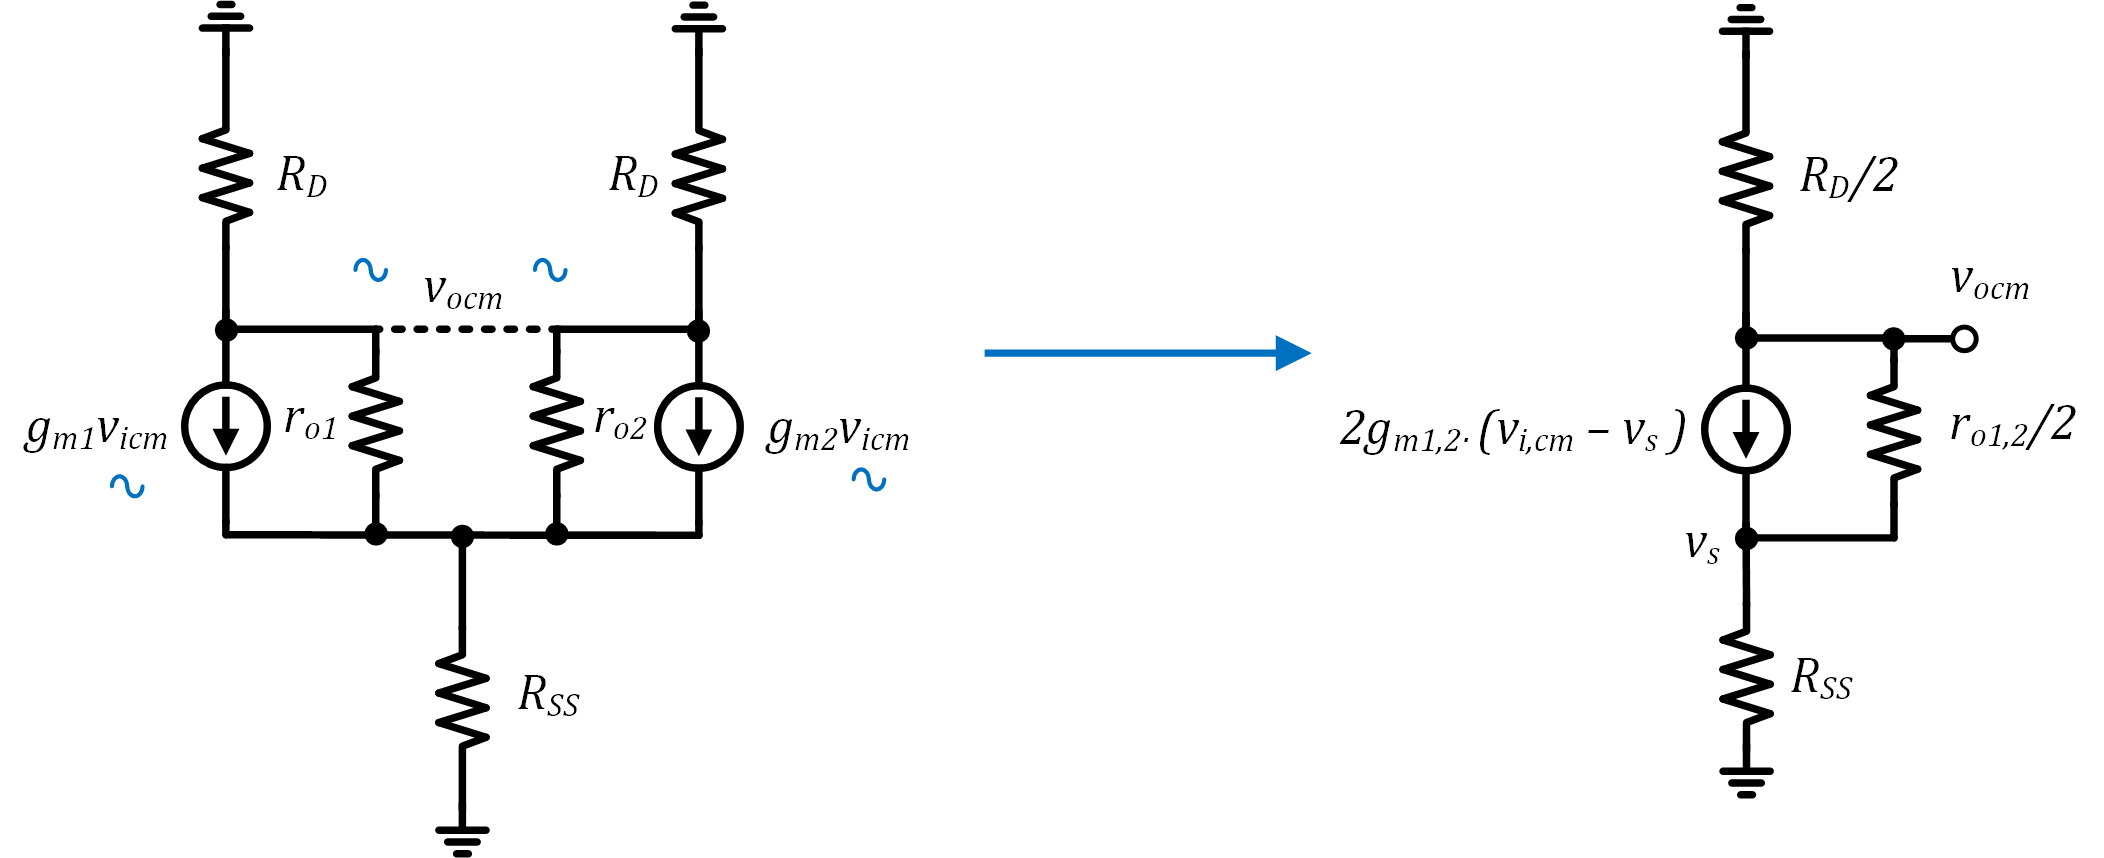
\includegraphics{CM_parallel_circuit.png}
\caption{CM\_parallel\_circuit.png}
\end{figure}

    \begin{itemize}
\tightlist
\item
  Common-mode inputs and outputs are, by definition, equal to each other
\item
  As a result, common-mode signals can be viewed as virtual
  short-circuits between respective nodes
\item
  The result is two \emph{parallel} amplifiers that can be combined to
  form a single ``common-mode amplifier''
\end{itemize}

    \hypertarget{common-mode-gain}{%
\subsection{Common-mode gain}\label{common-mode-gain}}

    \begin{figure}
\centering
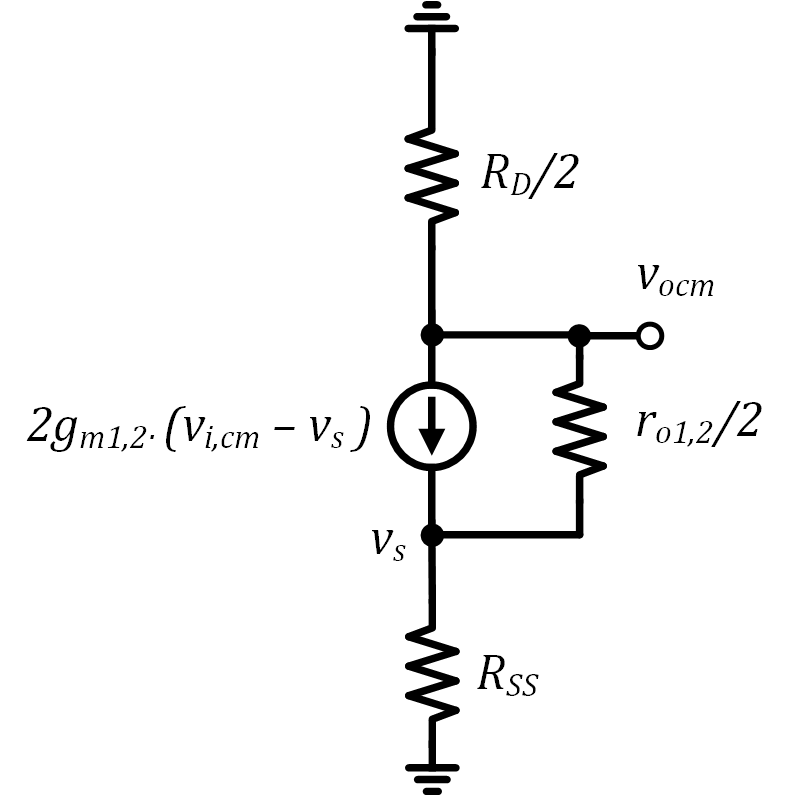
\includegraphics{CM_amplifier.png}
\caption{CM\_amplifier.png}
\end{figure}

    \begin{itemize}
\tightlist
\item
  The equivalent transconductance is given by
\end{itemize}

\begin{equation}
G_m = \dfrac{2g_{m1,2}}{1+\dfrac{2R_{SS}}{r_o} + 2g_m R_{SS}} \approx \dfrac{1}{R_{SS}}
\end{equation}

\begin{itemize}
\tightlist
\item
  The output resistance is
\end{itemize}

\begin{equation}
R_o \approx \dfrac{R_D}{2}
\end{equation}

\begin{itemize}
\tightlist
\item
  The common-mode gain is thus
\end{itemize}

\begin{equation}
\boxed{ A_{v,CM} = \dfrac{v_{ocm}}{v_{icm}} = -G_mR_o \approx \dfrac{-R_D}{2R_{SS}} }
\end{equation}

    \begin{itemize}
\tightlist
\item
  Common-mode circuit is a source-degenerated stage with degeneration
  resistance \(R_{SS}\)
\item
  \(R_{SS}\), since it is the output resistance of a current source,
  should be large
\item
  As a result, common-mode gain is much smaller than differential gain
\end{itemize}

    \hypertarget{common-mode-to-differential-gain}{%
\subsection{Common-mode-to-differential
gain}\label{common-mode-to-differential-gain}}

    \begin{figure}
\centering
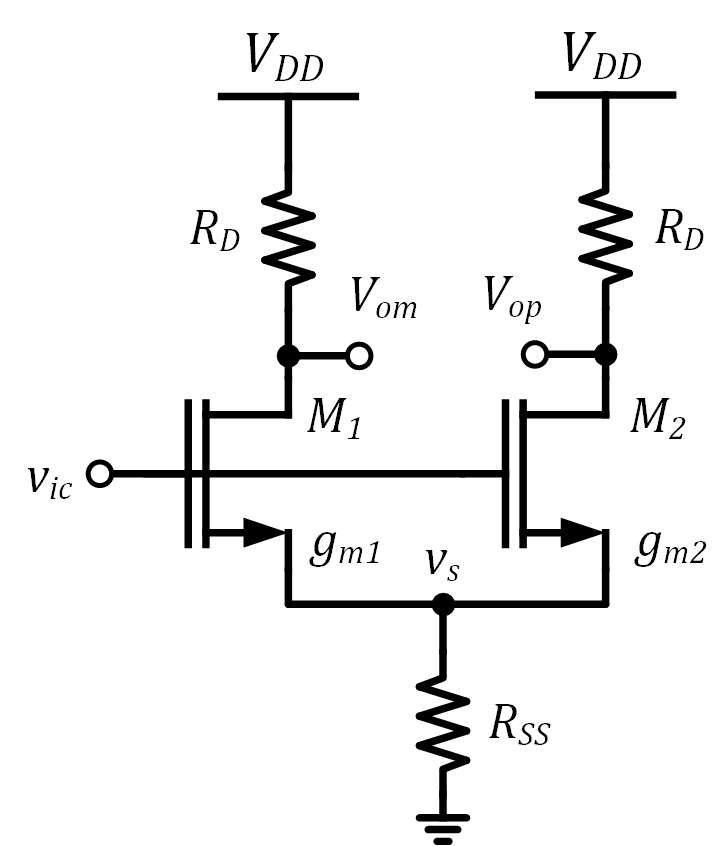
\includegraphics{CM_DM_mismatch.png}
\caption{CM\_DM\_mismatch.png}
\end{figure}

    \begin{itemize}
\item
  Of somewhat greater interest is the conversion of common-mode inputs
  to differential outputs
\item
  Mismatches in the threshold voltages and drain currents of \(M_1\) and
  \(M_2\) result in a differential output that varies with changes in
  the input common-mode level
\item
  This ``common-mode-to-differential conversion'' corrupts the
  differential output and degrades precision
\item
  Let's take a look at how an input common-mode change affects the
  differential output
\end{itemize}

    \begin{itemize}
\tightlist
\item
  Source degeneration reduces the effective \emph{common-mode}
  transconductances of \(M_1\) and \(M_2\) to
\end{itemize}

\begin{equation} 
G_{m1,2} = \dfrac{g_{m1,2}}{(g_{m1} + g_{m2})R_{SS} + 1}
\end{equation}

\begin{itemize}
\tightlist
\item
  Due to the mismatch between \(g_{m1}\) and \(g_{m2}\), this gives rise
  to a differential output voltage of
\end{itemize}

\begin{equation}
v_{od} = v_{op} - v_{om} = \dfrac{g_{m1} - g_{m2}}{(g_{m1} + g_{m2})R_{SS} + 1}R_D v_{ic}
\end{equation}

\begin{itemize}
\tightlist
\item
  The circuit thus converts input common-mode variations to a
  differential error given by a factor given by
\end{itemize}

\begin{equation}
A_{cm-dm} = \dfrac{\Delta g_m R_D}{(g_{m1} + g_{m2})R_{SS} + 1}
\end{equation}

\begin{itemize}
\tightlist
\item
  Comparison of \(A_{cm-dm}\) to the circuit's differential gain gives
  us the common-mode rejection ratio (CMRR)
\end{itemize}

\begin{equation}
CMRR = \left| \dfrac{A_{dm}}{A_{cm-dm}} \right| \approx \dfrac{g_m}{\Delta g_m}(2g_{m}R_{SS} + 1)
\end{equation}

    \hypertarget{differential-pair-with-active-mirror-load-5-transistor-ota}{%
\subsection{Differential pair with active mirror load (5-transistor
OTA)}\label{differential-pair-with-active-mirror-load-5-transistor-ota}}

    \begin{figure}
\centering
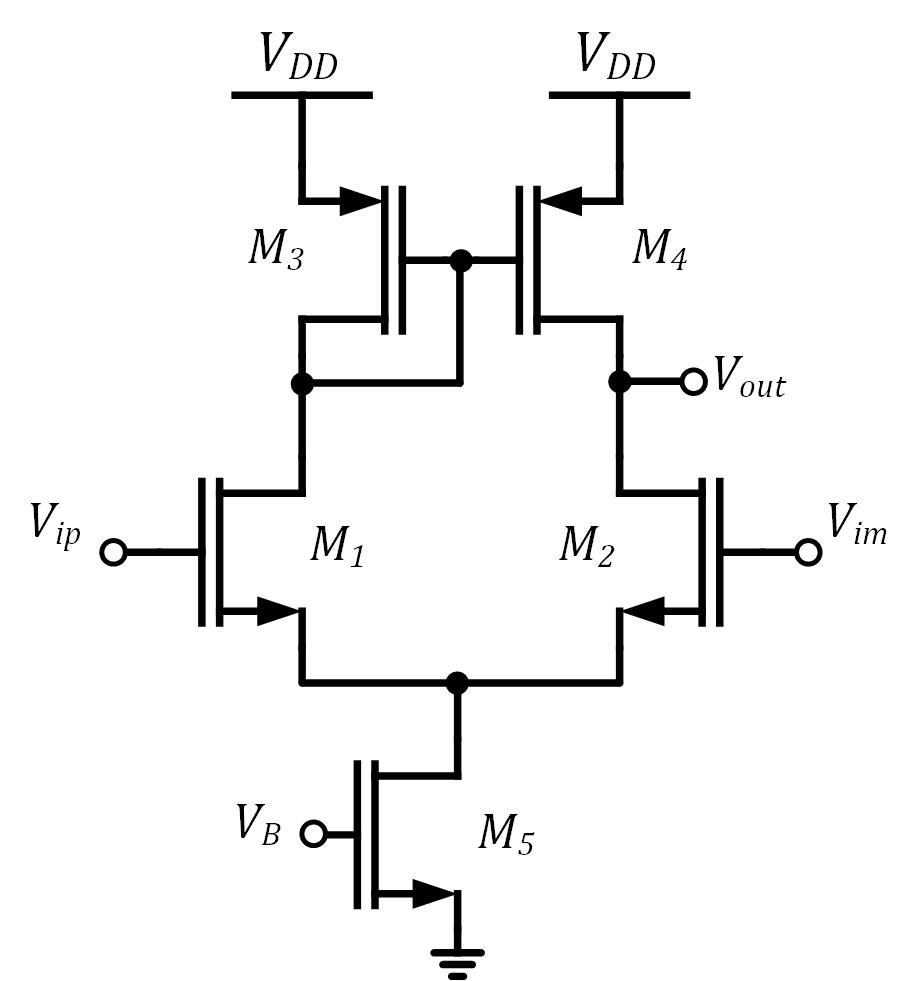
\includegraphics{diff_pair_active_mirror_load.png}
\caption{diff\_pair\_active\_mirror\_load.png}
\end{figure}

    \begin{itemize}
\tightlist
\item
  Bias is current set by \(M_5\), such that
\end{itemize}

\begin{equation} 
I_{D1} = I_{D2} = \dfrac{I_{D5}}{2}
\end{equation}

\begin{itemize}
\tightlist
\item
  Assuming \(I_{D1} = I_{D2}\) and \(V_{ip} = V_{im}\)
\end{itemize}

\begin{equation}
V_{out} \approx V_{DD} - V_{SG3}
\end{equation}

    \begin{itemize}
\tightlist
\item
  Differential pair with single-ended output that comprises the core of
  most operational amplifiers
\item
  ``Tail'' current source \(M_5\) biases the amplifier (may also be a
  cascode current source)
\item
  ``Active'' current mirror of \(M_3\), \(M_4\) converts differential
  signal current into a single-ended output
\end{itemize}

    \hypertarget{small-signal-model}{%
\subsection{Small-signal model}\label{small-signal-model}}

    \begin{figure}
\centering
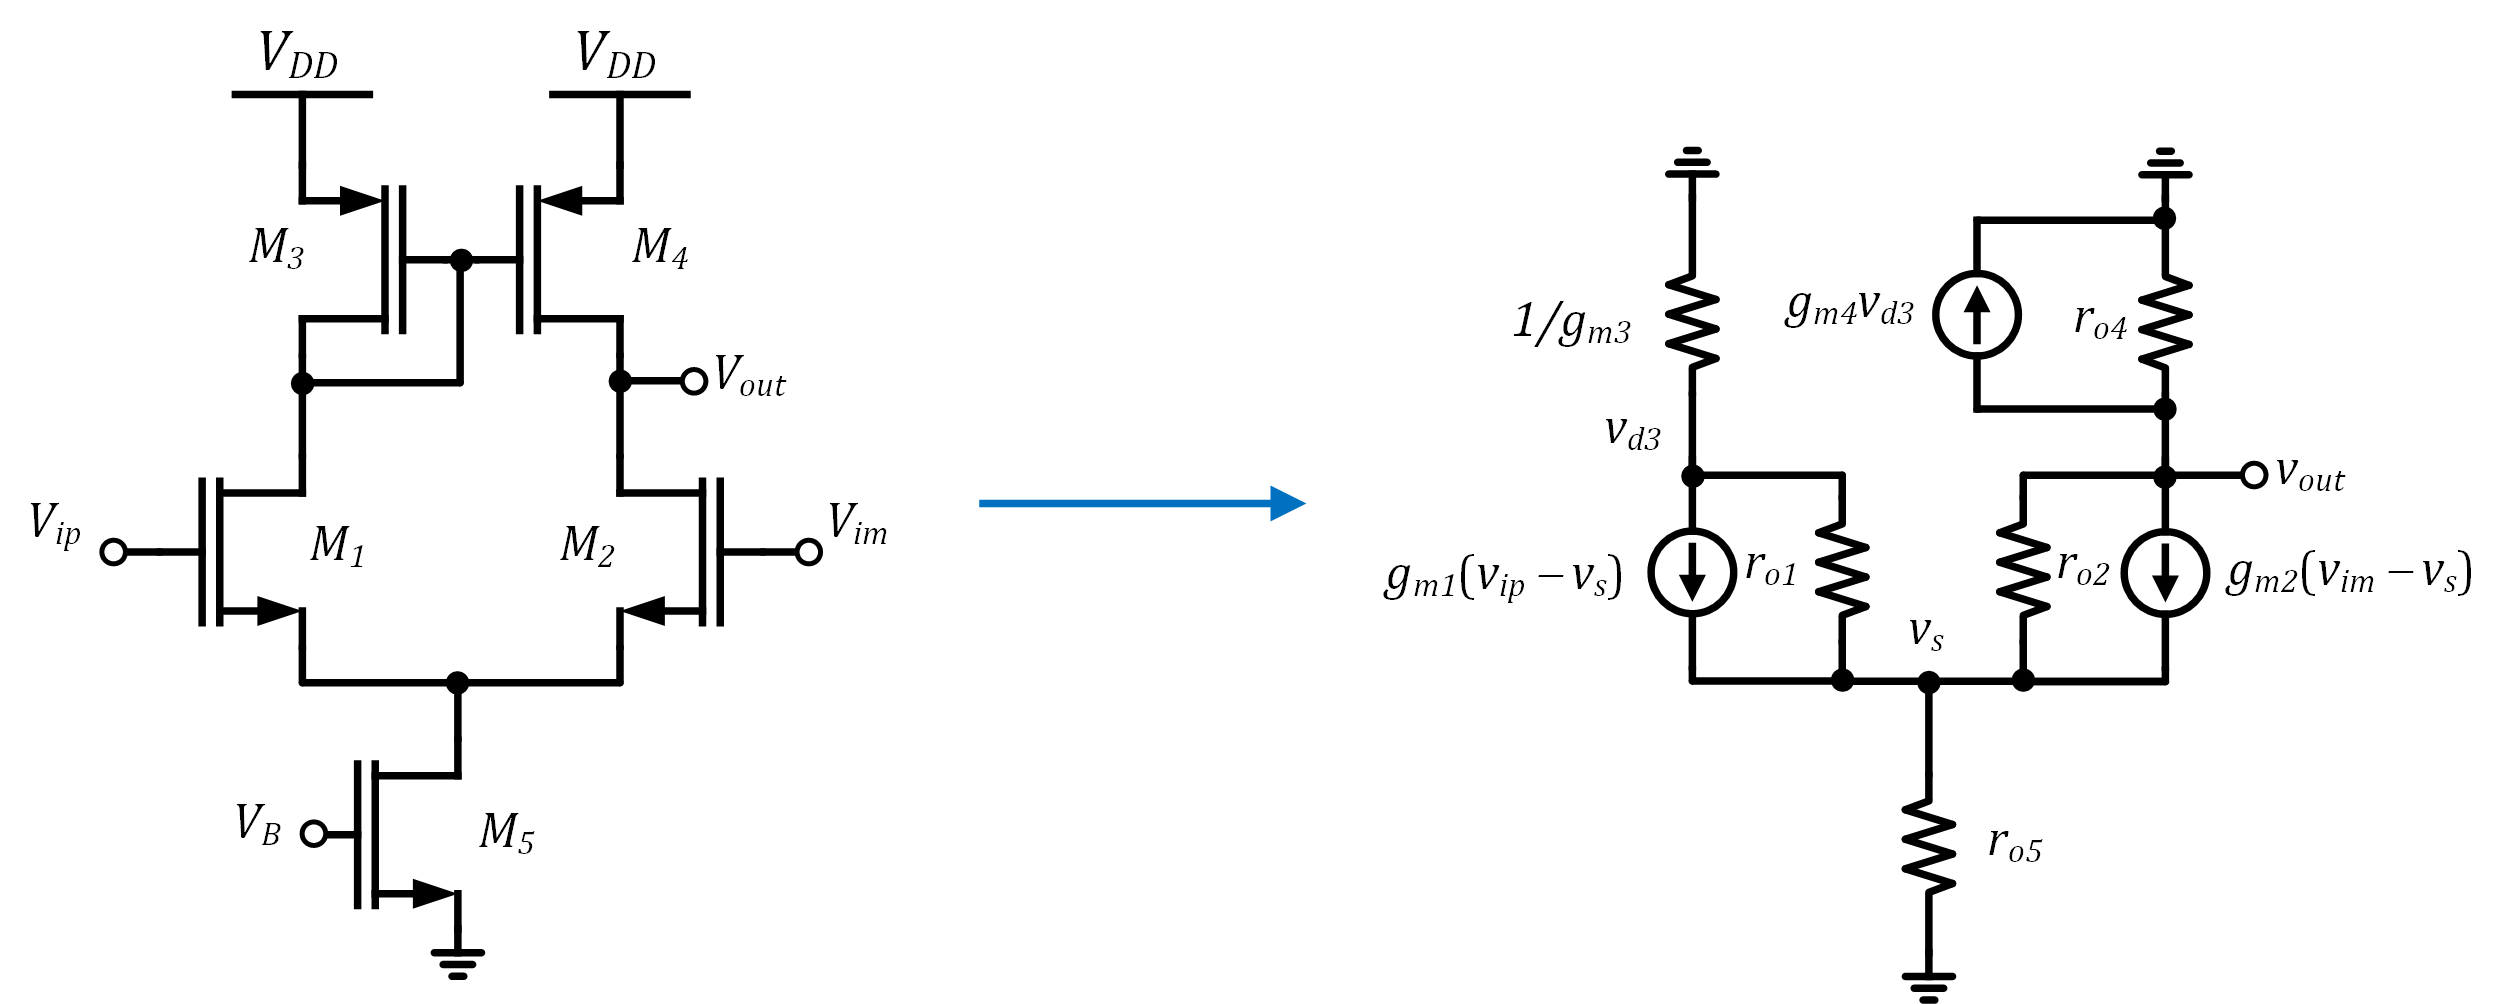
\includegraphics{diff_pair_mirror_load_small_signal.png}
\caption{diff\_pair\_mirror\_load\_small\_signal.png}
\end{figure}

    \begin{itemize}
\tightlist
\item
  In a small-signal sense, diode-connected \(M_3\) behaves as a
  resistance \(1/g_{m3}\)
\item
  Current mirror copies \(M_3\)'s small-signal current to \(M_4\)
\item
  Impedances looking into drains of \(M_1\) and \(M_2\) are not the
  same, so the circuit is somewhat assymetric
\end{itemize}

    \hypertarget{small-signal-analysis}{%
\subsection{Small-signal analysis}\label{small-signal-analysis}}

    \begin{figure}
\centering
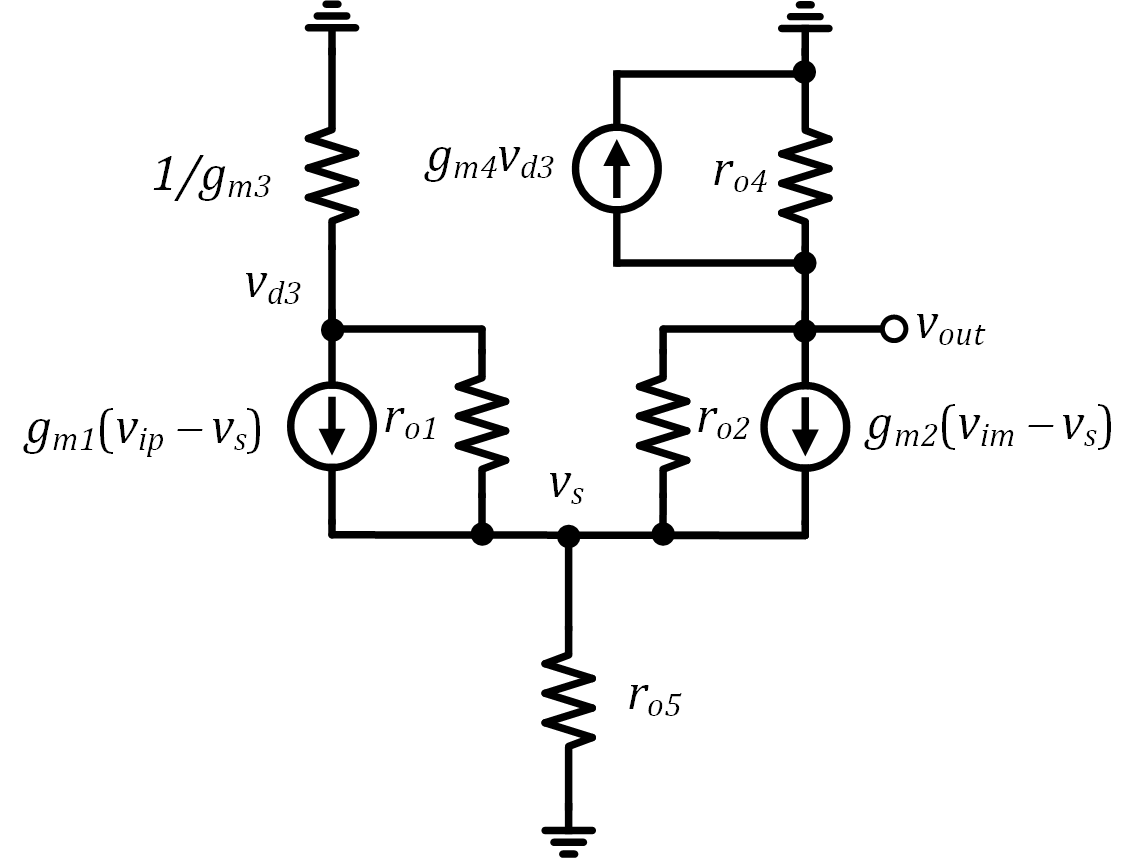
\includegraphics{active_mirror_small_signal.png}
\caption{active\_mirror\_small\_signal.png}
\end{figure}

    \begin{equation}
v_s \approx 0
\end{equation}

\begin{equation}
v_{d3} \approx -\dfrac{g_{m1}}{g_{m3}}v_{ip}
\end{equation}

\begin{equation}
g_{m3} = g_{m4}
\end{equation}

\begin{equation}
\boxed{g_{m4}v_{d3} \approx -g_{m4}\dfrac{g_{m1}}{g_{m3}}v_{ip} = -g_{m1}v_{ip}}
\end{equation}

    \begin{itemize}
\tightlist
\item
  \(v_s\) again acts as a virtual ground due to the symmetry of the
  circuit
\item
  Neglecting \(r_{o1}\) and \(r_{o3}\), the current in \(M_3\) is equal
  to \(g_{m1} (v_{ip} - v_s)\)
\item
  The ``active'' current mirror mirrors this current through \(M_4\)'s
  transconductance, \(g_{m4}\)
\item
  The output current is thus the \emph{difference} of \(g_{m2}v_{im}\)
  and \(g_{m1}v_{ip}\)
\end{itemize}

    \hypertarget{differential-transconductance-gm}{%
\subsection{Differential transconductance
(Gm)}\label{differential-transconductance-gm}}

    \begin{figure}
\centering
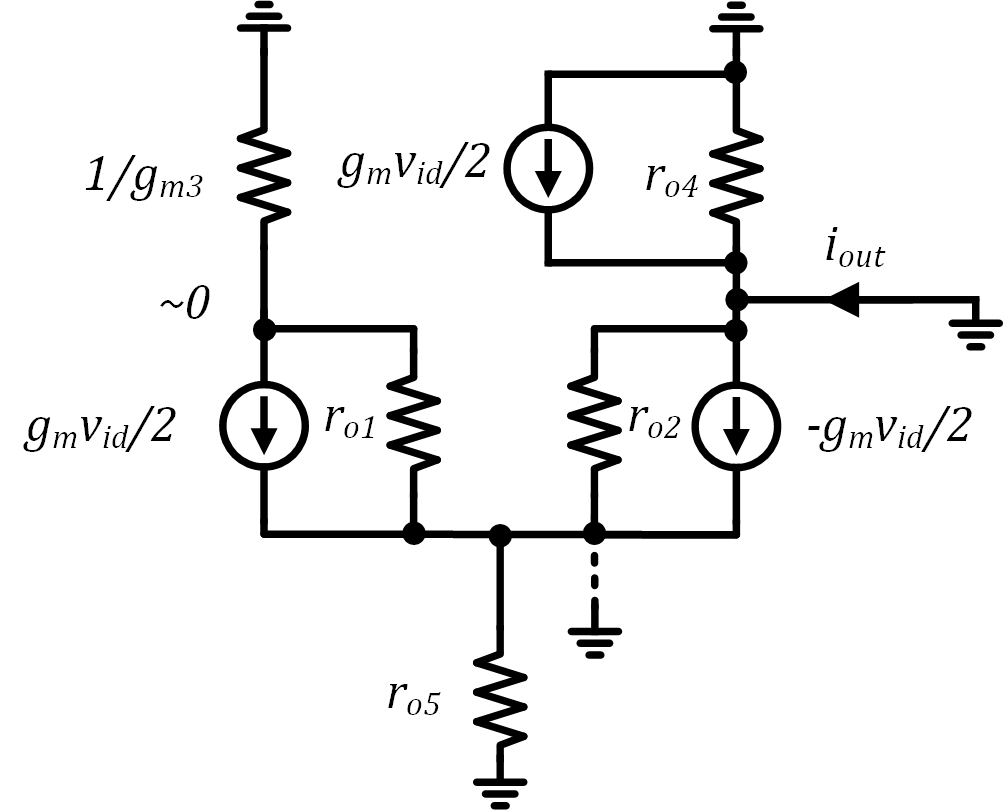
\includegraphics{active_mirror_Gm.png}
\caption{active\_mirror\_Gm.png}
\end{figure}

    \begin{itemize}
\tightlist
\item
  The short-circuit current is given by
\end{itemize}

\begin{align}
i_{out} &\approx -g_{m1,2} \left( \dfrac{v_{id}}{2} + \dfrac{v_{id}}{2} \right) \\
&\approx -g_{m1,2} v_{id} \\
\end{align}

\begin{itemize}
\tightlist
\item
  As before, \(G_m\) is determined by taking the ratio of the
  short-circuit current to the input voltage
\end{itemize}

\begin{equation}
\boxed{G_m = \dfrac{i_{out}}{v_{id}} \approx -g_{m1,2}}
\end{equation}

    \begin{itemize}
\tightlist
\item
  The small-signal voltage at drain of \(M_1\) is small
  (i.e.~approximately \(0\))
\item
  The circuit is \emph{approximately} symmetric, since the current
  through \(r_{o1}\) is small relative to the contribution from
  \(g_{m1}\)
\item
  The source of \(M_1\), \(M_2\) can thus be viewed as a virtual ground
\end{itemize}

    \hypertarget{output-resistance-ro}{%
\subsection{Output resistance (Ro)}\label{output-resistance-ro}}

    \begin{figure}
\centering
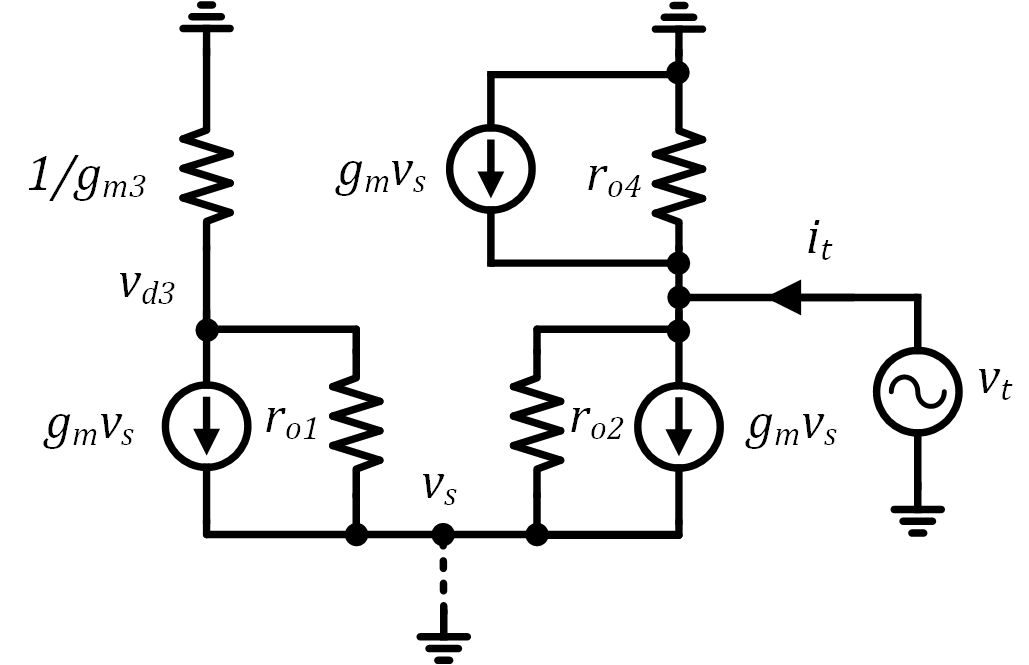
\includegraphics{active_mirror_Ro.png}
\caption{active\_mirror\_Ro.png}
\end{figure}

    \begin{itemize}
\tightlist
\item
  Due to the virtual ground, \(v_s \approx 0\), and \(i_t\) is given by
\end{itemize}

\begin{equation}
i_t \approx \dfrac{v_t}{r_{o2}} + \dfrac{v_t}{r_{o4}}
\end{equation}

\begin{itemize}
\tightlist
\item
  The output resistance is determined as the ratio \(v_t/i_t\)
\end{itemize}

\begin{equation}
\boxed{ R_o = \dfrac{v_t}{i_t} \approx r_{o2}||r_{o4} }
\end{equation}

    \begin{itemize}
\tightlist
\item
  Negligible differential current flows through tail resistance
  (\(r_{o5}\)), making it (approximately) a virtual ground
\item
  Output resistance is the parallel combination of \(r_{o2}\) and
  \(r_{o4}\)
\end{itemize}

    \hypertarget{differential-gain}{%
\subsection{Differential gain}\label{differential-gain}}

    \begin{figure}
\centering
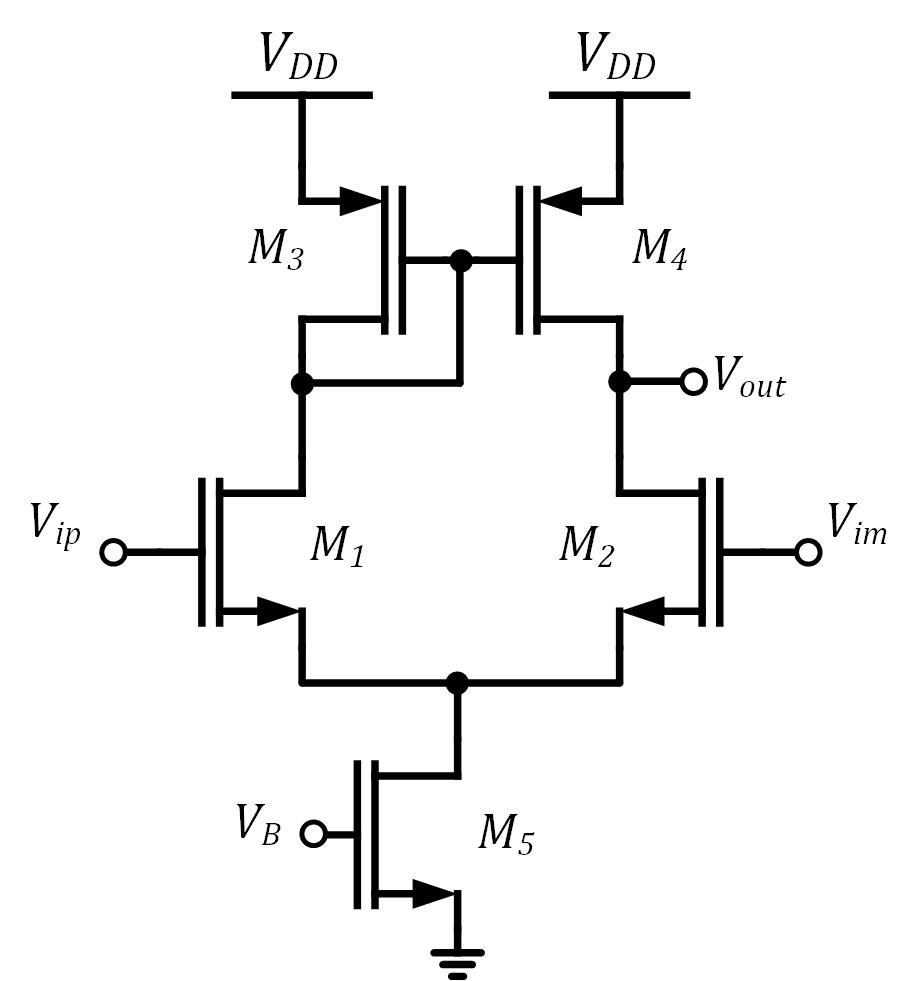
\includegraphics{diff_pair_active_mirror_load.png}
\caption{diff\_pair\_active\_mirror\_load.png}
\end{figure}

    \begin{itemize}
\tightlist
\item
  The differential transconductance and output resistance of the
  amplifier are given by
\end{itemize}

\begin{equation}
G_m \approx -g_{m1,2}
\end{equation}

\begin{equation}
R_o = r_{o1}||r_{o4}
\end{equation}

\begin{itemize}
\tightlist
\item
  The differential gain is thus
\end{itemize}

\begin{equation}
\boxed{A_{v,d} = -G_m R_o \approx g_{m1,2}\cdot r_{o1}||r_{o4}}
\end{equation}

    \begin{itemize}
\tightlist
\item
  Differential input, single-ended output amplifier with \(G_m R_o\)
  gain that forms the core of opamps and OTAs
\item
  In the ideal case, \(R_o \rightarrow \infty\), so this amplifier is
  often viewed as an operational transconductance amplifier (OTA)
\item
  Due to mismatched impedances at drain of \(M_1\) and \(M_2\),
  common-mode rejection is inherently imperfect
\end{itemize}

    \hypertarget{telescopic-cascode-ota}{%
\subsection{``Telescopic'' cascode OTA}\label{telescopic-cascode-ota}}

    \begin{figure}
\centering
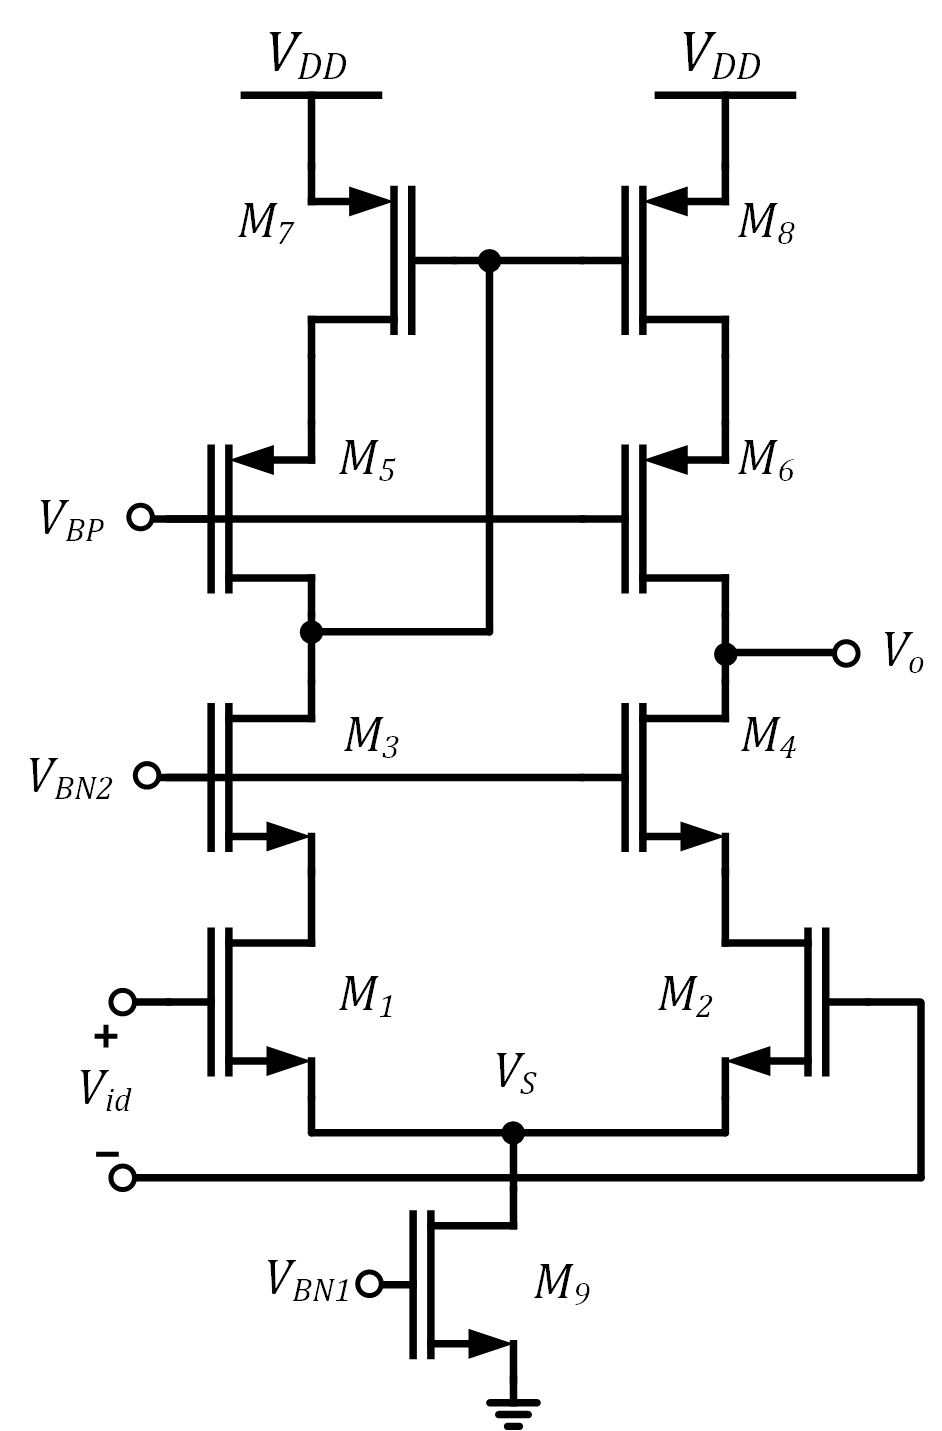
\includegraphics{telescopic_cascode_OTA.png}
\caption{telescopic\_cascode\_OTA.png}
\end{figure}

    \begin{itemize}
\item
  Analogous structure to the 5-transistor OTA, with cascoding
\item
  \(V_{BN1}\) and \(V_{BP}\) are generated using the biasing structures
  discussed previously
\item
  \(V_{BN2}\) can be set relative to \(V_S\) (dyanmic biasing),
  increasing the input range of the OTA
\item
  The gain is given approximately by
\end{itemize}

\begin{align}
A_v  = \dfrac{V_o}{V_{id}} &= -G_m R_o\\
\\
&= \boxed{-g_{m1,2}\cdot( g_{m4}r_{o4}r_{o2}|| g_{m6}r_{o6}r_{o8})}\\
\end{align}

    \hypertarget{folded-cascode-ota}{%
\subsection{``Folded'' cascode OTA}\label{folded-cascode-ota}}

    \begin{figure}
\centering
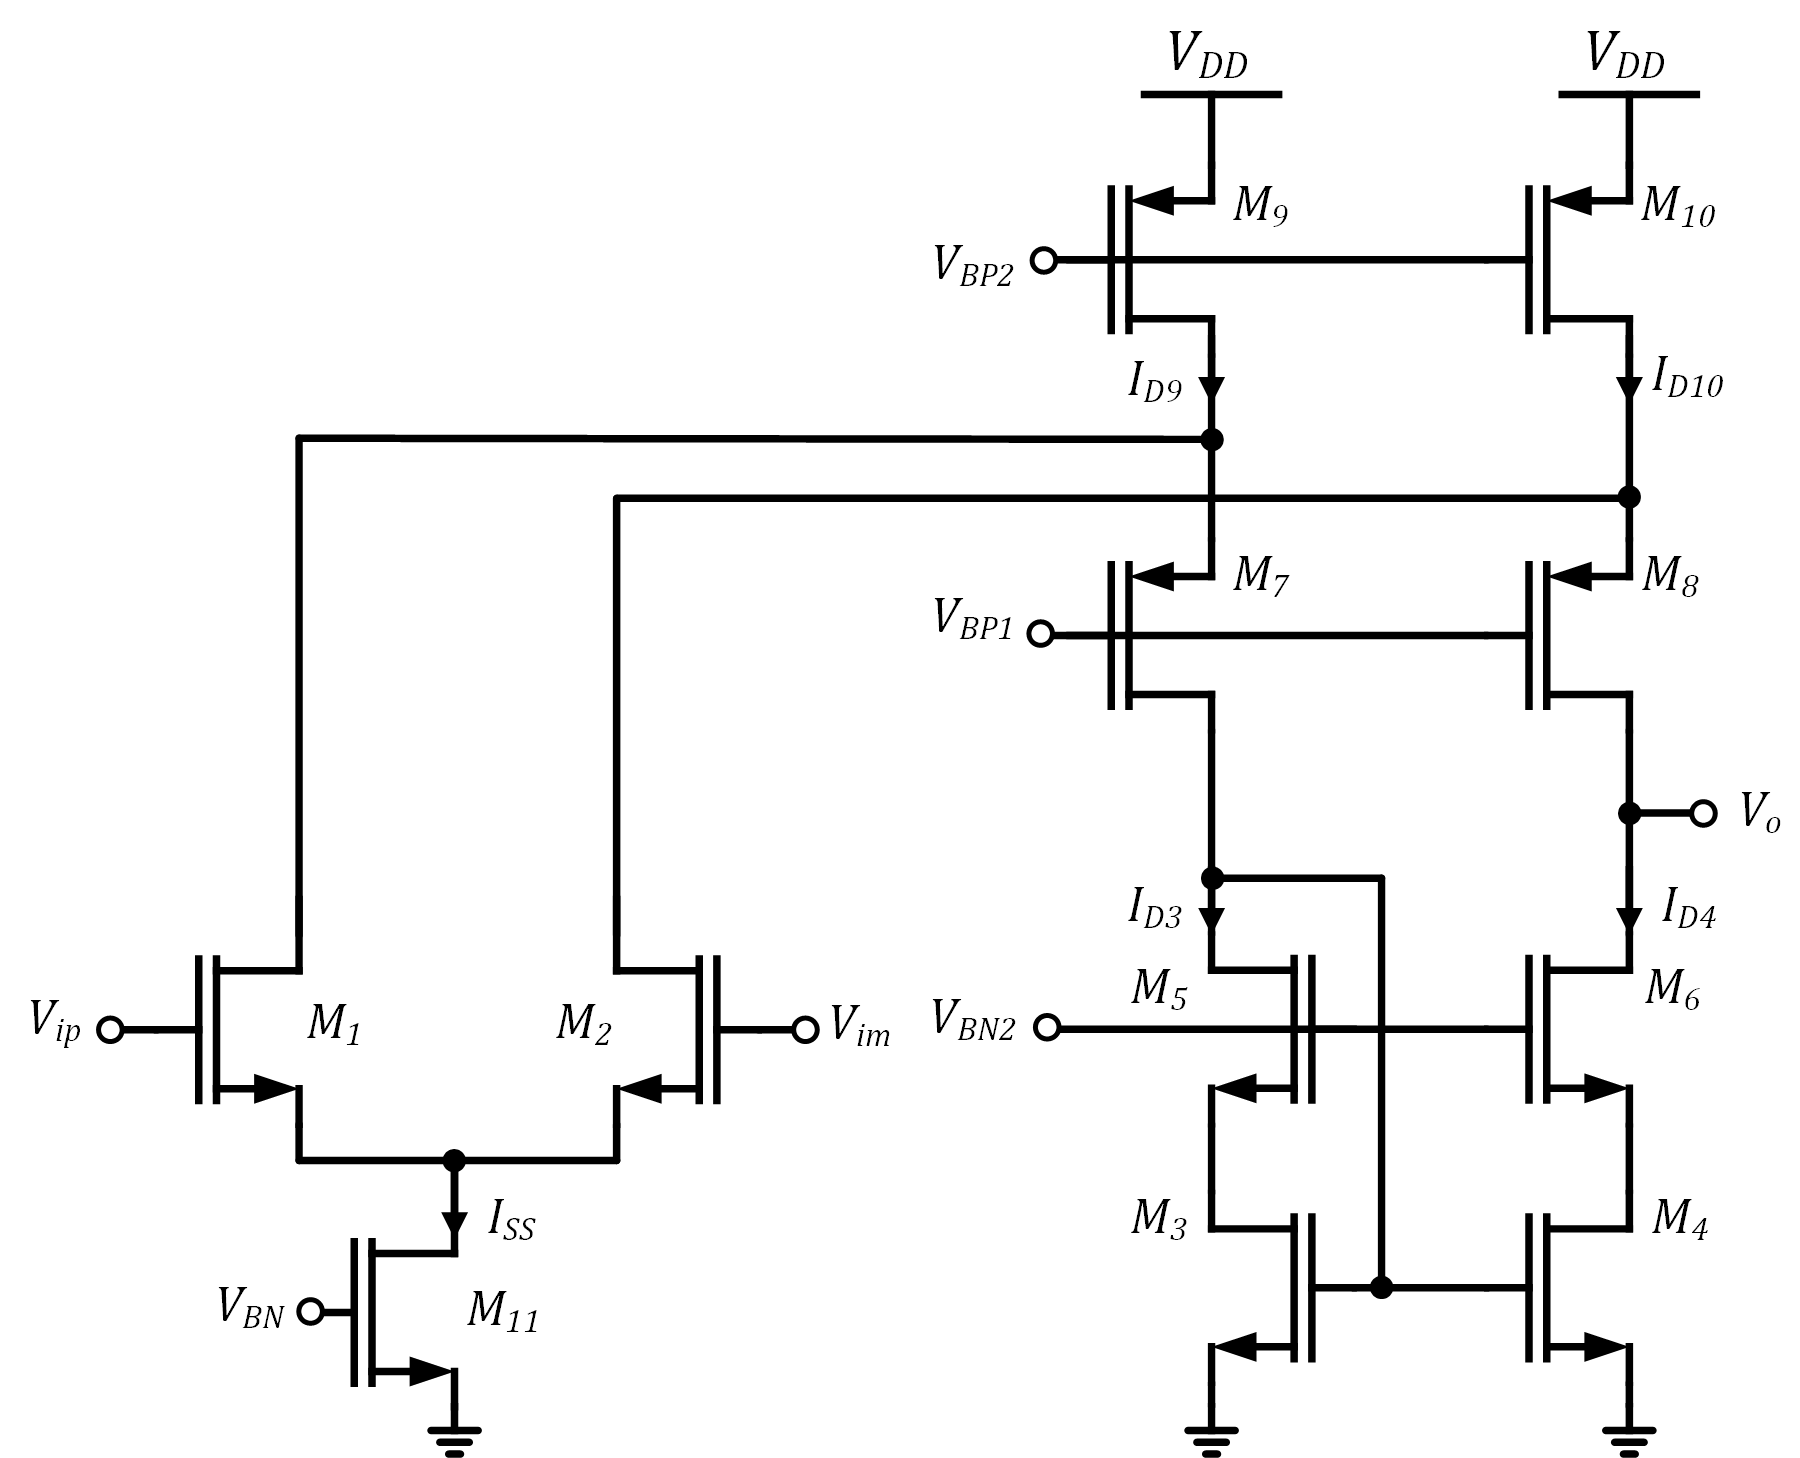
\includegraphics{folded_cascode_OTA.png}
\caption{folded\_cascode\_OTA.png}
\end{figure}

    \begin{itemize}
\item
  Cascode structure enabling greater output swing than the telescopic
  OTA
\item
  \(V_{BN}\), \(V_{BN2}\), \(V_{BP1}\), and \(V_{BP2}\) generated using
  current mirrors and cascode bias schemes
\item
  \(M_9\) and \(M_{10}\) supply current to both halves of the OTA:
\end{itemize}

\begin{equation}
I_{D9,10} = \dfrac{I_{SS}}{2} + I_{D3,4}
\end{equation}

\begin{itemize}
\tightlist
\item
  The gain is given by
\end{itemize}

\begin{align}
A_v  = \dfrac{V_o}{V_{id}} &= -G_m R_o\\
\\
&= \boxed{-g_{m1,2}\cdot( g_{m6}r_{o4}r_{o6}|| g_{m8}r_{o10}r_{o8})}\\
\end{align}

    \hypertarget{summary}{%
\subsection{Summary}\label{summary}}

    \begin{itemize}
\tightlist
\item
  Differential signaling provides advantages with respect to common-mode
  noise, signal swing, and SNR
\item
  Differential pairs are current-biased using MOS current sources,
  enabling independent design of bias point and gain
\item
  High-gain opamps and OTAs are based on the 5-transistor OTA, which
  uses an ``active'' current mirror to achieve differential operation in
  the current domain
\item
  Cascode versions of the 5-transistor OTA increase gain, and form the
  core of most opamps
\end{itemize}


    % Add a bibliography block to the postdoc
    
    
    
\end{document}
